%!TEX root = ../thesis.tex

\chapter{中国东南部深对流对痕量气体垂直分布的影响}

\section{模式设置}

\subsection{气象及化学设置}

该研究使用的WRF-Chem版本号为4.1.4,气象条件的初始场和边界场来自1小时分辨率的欧洲中心大气再分析数据(ERA5,\citet{Hersbach.2020})。
模式的垂直分层为75层,对流层顶设置为50 hPa,嵌套区域如图\ref{fig:domains_china}所示。
微物理过程使用WSM6方案\citep{Hong.2006a},而短波和长波辐射使用RRTMG方案\citep{Iacono.2008},陆面过程由Noah方案模拟\citep{Koren.1999}。
但是,我们使用不同的边界层参数化来模拟两次对流个例,2019年的个例使用YSU方案\citep{Hong.2006},而2020年的个例使用QNSE方案\citep{Sukoriansky.2005}。
闪电部分未使用参数化,用闪电同化代替,详见\ref{sect:lightning_assimilation}节。

化学初始场和边界场采用整个大气社区气候模型(WACCM,\url{https://www.acom.ucar.edu/waccm/})的输出数据。
其中2020年个例的初始O$_3$廓线使用臭氧探空仪观测所得的O$_3$廓线。
人为排放使用2016年中国多分辨率排放清单 (MEIC,\url{http://www.meicmodel.org/})1.3版驱动,生物排放采用来自自然界的气体和气溶胶排放模型(MEGAN;\citet{Guenther.2006})。
化学机理使用气相化学的臭氧和相关化学示踪剂模式(MOZART)和气溶胶的Goddard化学气溶胶辐射和传输(GOCART)模式\citep{Pfister.2011}。
其中光解方案采用基于云光学厚度(cloud\_fraction$^{1.5}$)的新 TUV(对流层紫外线和可见光)方案,即光解速率依赖于气溶胶和云。
此外,LNO的垂直廓线使用\citet{Ott.2010}的双峰型闪电NO(LNO)廓线\citep{Laughner.2017},而LNO和LNO$_2$廓线是指开启和关闭闪电选项的模拟之间垂直廓线的差异。
其中LNO$_x$参数化调整为每次闪电产生500 mol NO\citep{Zhu.2019}。

\begin{figure}[htbp]
\centering
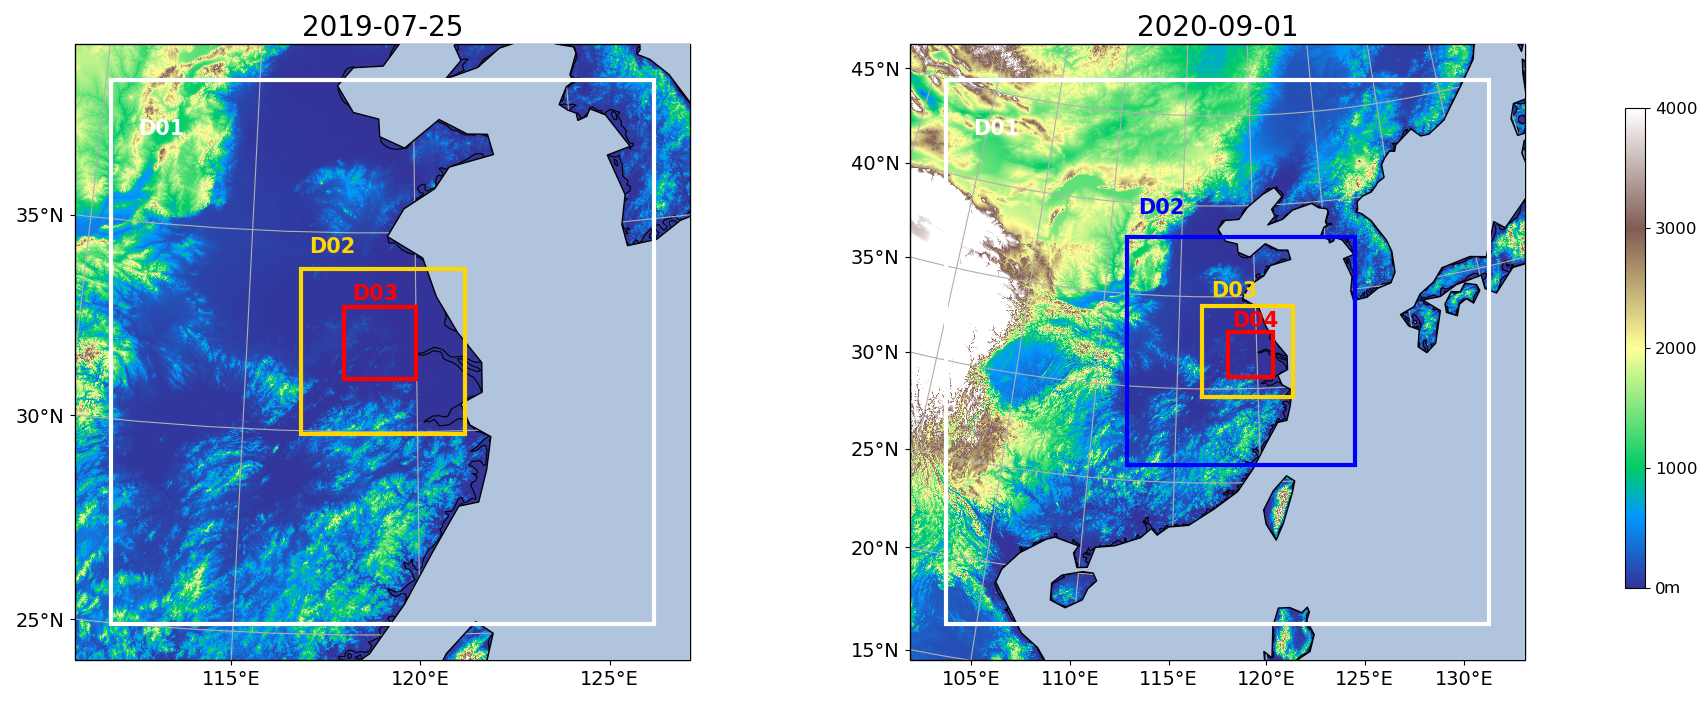
\includegraphics[width=0.9\textwidth]{./figures/domains_china.png}
\caption{2019年和2020年个例的WRF-Chem模拟区域和地形高度(m)图。
2019年个例的水平网格分辨率为15 km(D01)、3 km(D02)和 0.6 km(D03)。
对于2020年个例,分别为27 km(D01)、9 km(D02)、3 km(D03)和 1 km(D04)。\\
Figure \ref{fig:domains_china}. Domain and terrain height (m) of the WRF-Chem simulations for the 2019 and 2020 cases. The horizontal grid resolution of
domains for the 2019 case is 15 km (D01), 3 km (D02) and 0.6 km (D03). For the 2020 case, it is 27 km (D01), 9 km (D02), 3 km (D03),
and 1 km (D04).}
\label{fig:domains_china}
\end{figure}

\subsection{闪电同化} \label{sect:lightning_assimilation}

为了更准确地模拟出对流和LNO$_x$,我们将闪电数据同化应用于 WRF-Chem。
闪电数据同化方法详见\citet{Fierro.2012}和\citet{Li.2017b},主要步骤为在发生闪电所处网格的垂直恒温层间,增加水汽质量混合比。

\begin{equation} \label{eq:lda}
Q_{v}=A Q_{\mathrm{sat}}+B Q_{\mathrm{sat}} \tanh (C X)\left[1-\tanh \left(D Q_{g}^{\alpha}\right)\right]
\end{equation}

式(\ref{eq:lda})中,Q$_{sat}$ 为水汽饱和混合比(g kg$^{−1}$),Q$_g$为霰粒混合比(g kg$^{−1}$),X 为闪电频率。
本研究选择263.15 和 290.15 K作为恒温层的上下界限,其目的是为了让对流在行星边界层中快速扎根,因为对流层低层的Q$_v$更深\citep{Marchand.2014,Finney.2016,Li.2017b}。
参数设置参考\citet{Li.2017b}:A=0.94,B=0.2,C=0.001,D=0.25,α=2.2。
其中网格化的总闪数据通过WRF的辅助输入流进行每10分钟的读取。
例如,如果闪电同化开始于05:00 UTC,时间步长为10 min,则将05:00--05:10 UTC之间特定网格中所有闪电数相加作为此期间的贡献。
在下一个时间步长,闪电被归类为下一个新组。
因此,闪电数即闪电频率的密度(单位:flash每10 min 每dx km 每dy km),其中dx和dy分别是模型网格在x和y方向的分辨率。
如\citet{Fierro.2012}和\citet{Li.2017b}所述,这可以确保所有嵌套层中的闪电密度相同。
此外,闪电数也被直接同化进WRF-Chem中,该方法已被应用于社区多尺度空气质量(CMAQ,\citet{Kang.2019,Kang.2019a,Kang.2020}模式中。

\section{模式评估}

与雷达观测相比,2019年7月25日和2020年9月1日模拟的对流初生时间,较实际情况分别提前了60分钟和30分钟(图\ref{fig:comp_crf_2019}和图\ref{fig:comp_crf_2020}),闪电数据也以相同的时间间隔提前同化。
对于下文的结果比较,我们选择匹配的阶段而不是相同的时间。

2019年7月25日的热对流在初始时呈现为孤立的热泡,WRF-Chem再现了初始阶段孤立对流的位置和强度(图\ref{fig:comp_crf_2019}a和\ref{fig:comp_crf_2020}d)。
在05:40 UTC时,对流系统呈现东北-西南向,最大组合雷达反射率达到60 dBZ(图\ref{fig:comp_crf_2019}b),强度大于模拟的对流(最大组合雷达反射率为55 dBZ,图\ref{fig:comp_crf_2019}e)。
将模拟的对流核心区的雷达反射率垂直剖面与观测结果进行比较(图\ref{fig:comp_dbzcross_2019}),
虽然对流与雷达距离过远造成缺失数据较多,但是在未进行人工插值的条件下,孤立对流的水平和垂直结构仍大致显示。
模拟的45 dBZ等值线达到12 km,但由于10 km 以上的数据质量低,观测到的等值线仅达到10 km。

2020年9月1日观测到的飑线在北部初生,然后加强,并向观测点移动(图\ref{fig:comp_crf_2020})。
对流旺盛阶段(最大组合雷达反射率为60 dBZ)大致在05:50 UTC,与TROPOMI过境时间相符(图\ref{fig:comp_dbzcross_2020}b和e)。
虽然该飙线抵达的最高高度低于2019年的热对流,但对流层低层(2--8 km)的反射率更大更广(图\ref{fig:comp_dbzcross_2020})。
由于模拟的对流消散区偏离了雷达观测到的消散区,这导致与臭氧探空仪比较的区域设置在站点的西侧(图\ref{fig:comp_dbzcross_2020}c和f)。

在不同对流阶段所测的O$_3$和Q$_v$分布如图\ref{fig:ozonesonde_profile}所示。
一般来说,对流导致上对流层O$_3$和Q$_v$浓度增大,且增强的最大值所在区域为10--16 km 之间。
然而,2020年的个例观测显示对流层低层(2--8 km)的O$_3$有较大的增加。
此外,两个个例都存在双谷形状的O$_3$剖面,但高度不同:2019年的热对流个例为2 km和8 km,2020年的飑线为4 km和10 km。
尽管WRF-Chem模型倾向于分别低估2019年和2020年的下对流层和上对流层中的O$_3$浓度,但再现了详细的O$_3$垂直分布结构,故能用以分析对流影响O$_3$的机制。
共有三个来源可以解释上对流层O$_3$的增加:对流输送、化学反应和闪电直接产生的O$_3$。
本研究仅详细讨论前两个因素,因为闪电直接产生的O$_3$超出了本研究的范围,并且有限的观测和模式模拟结果显示其产量仍不确定\citep{Morris.2010,Ripoll.2014}。


\begin{figure}[htbp]
\centering
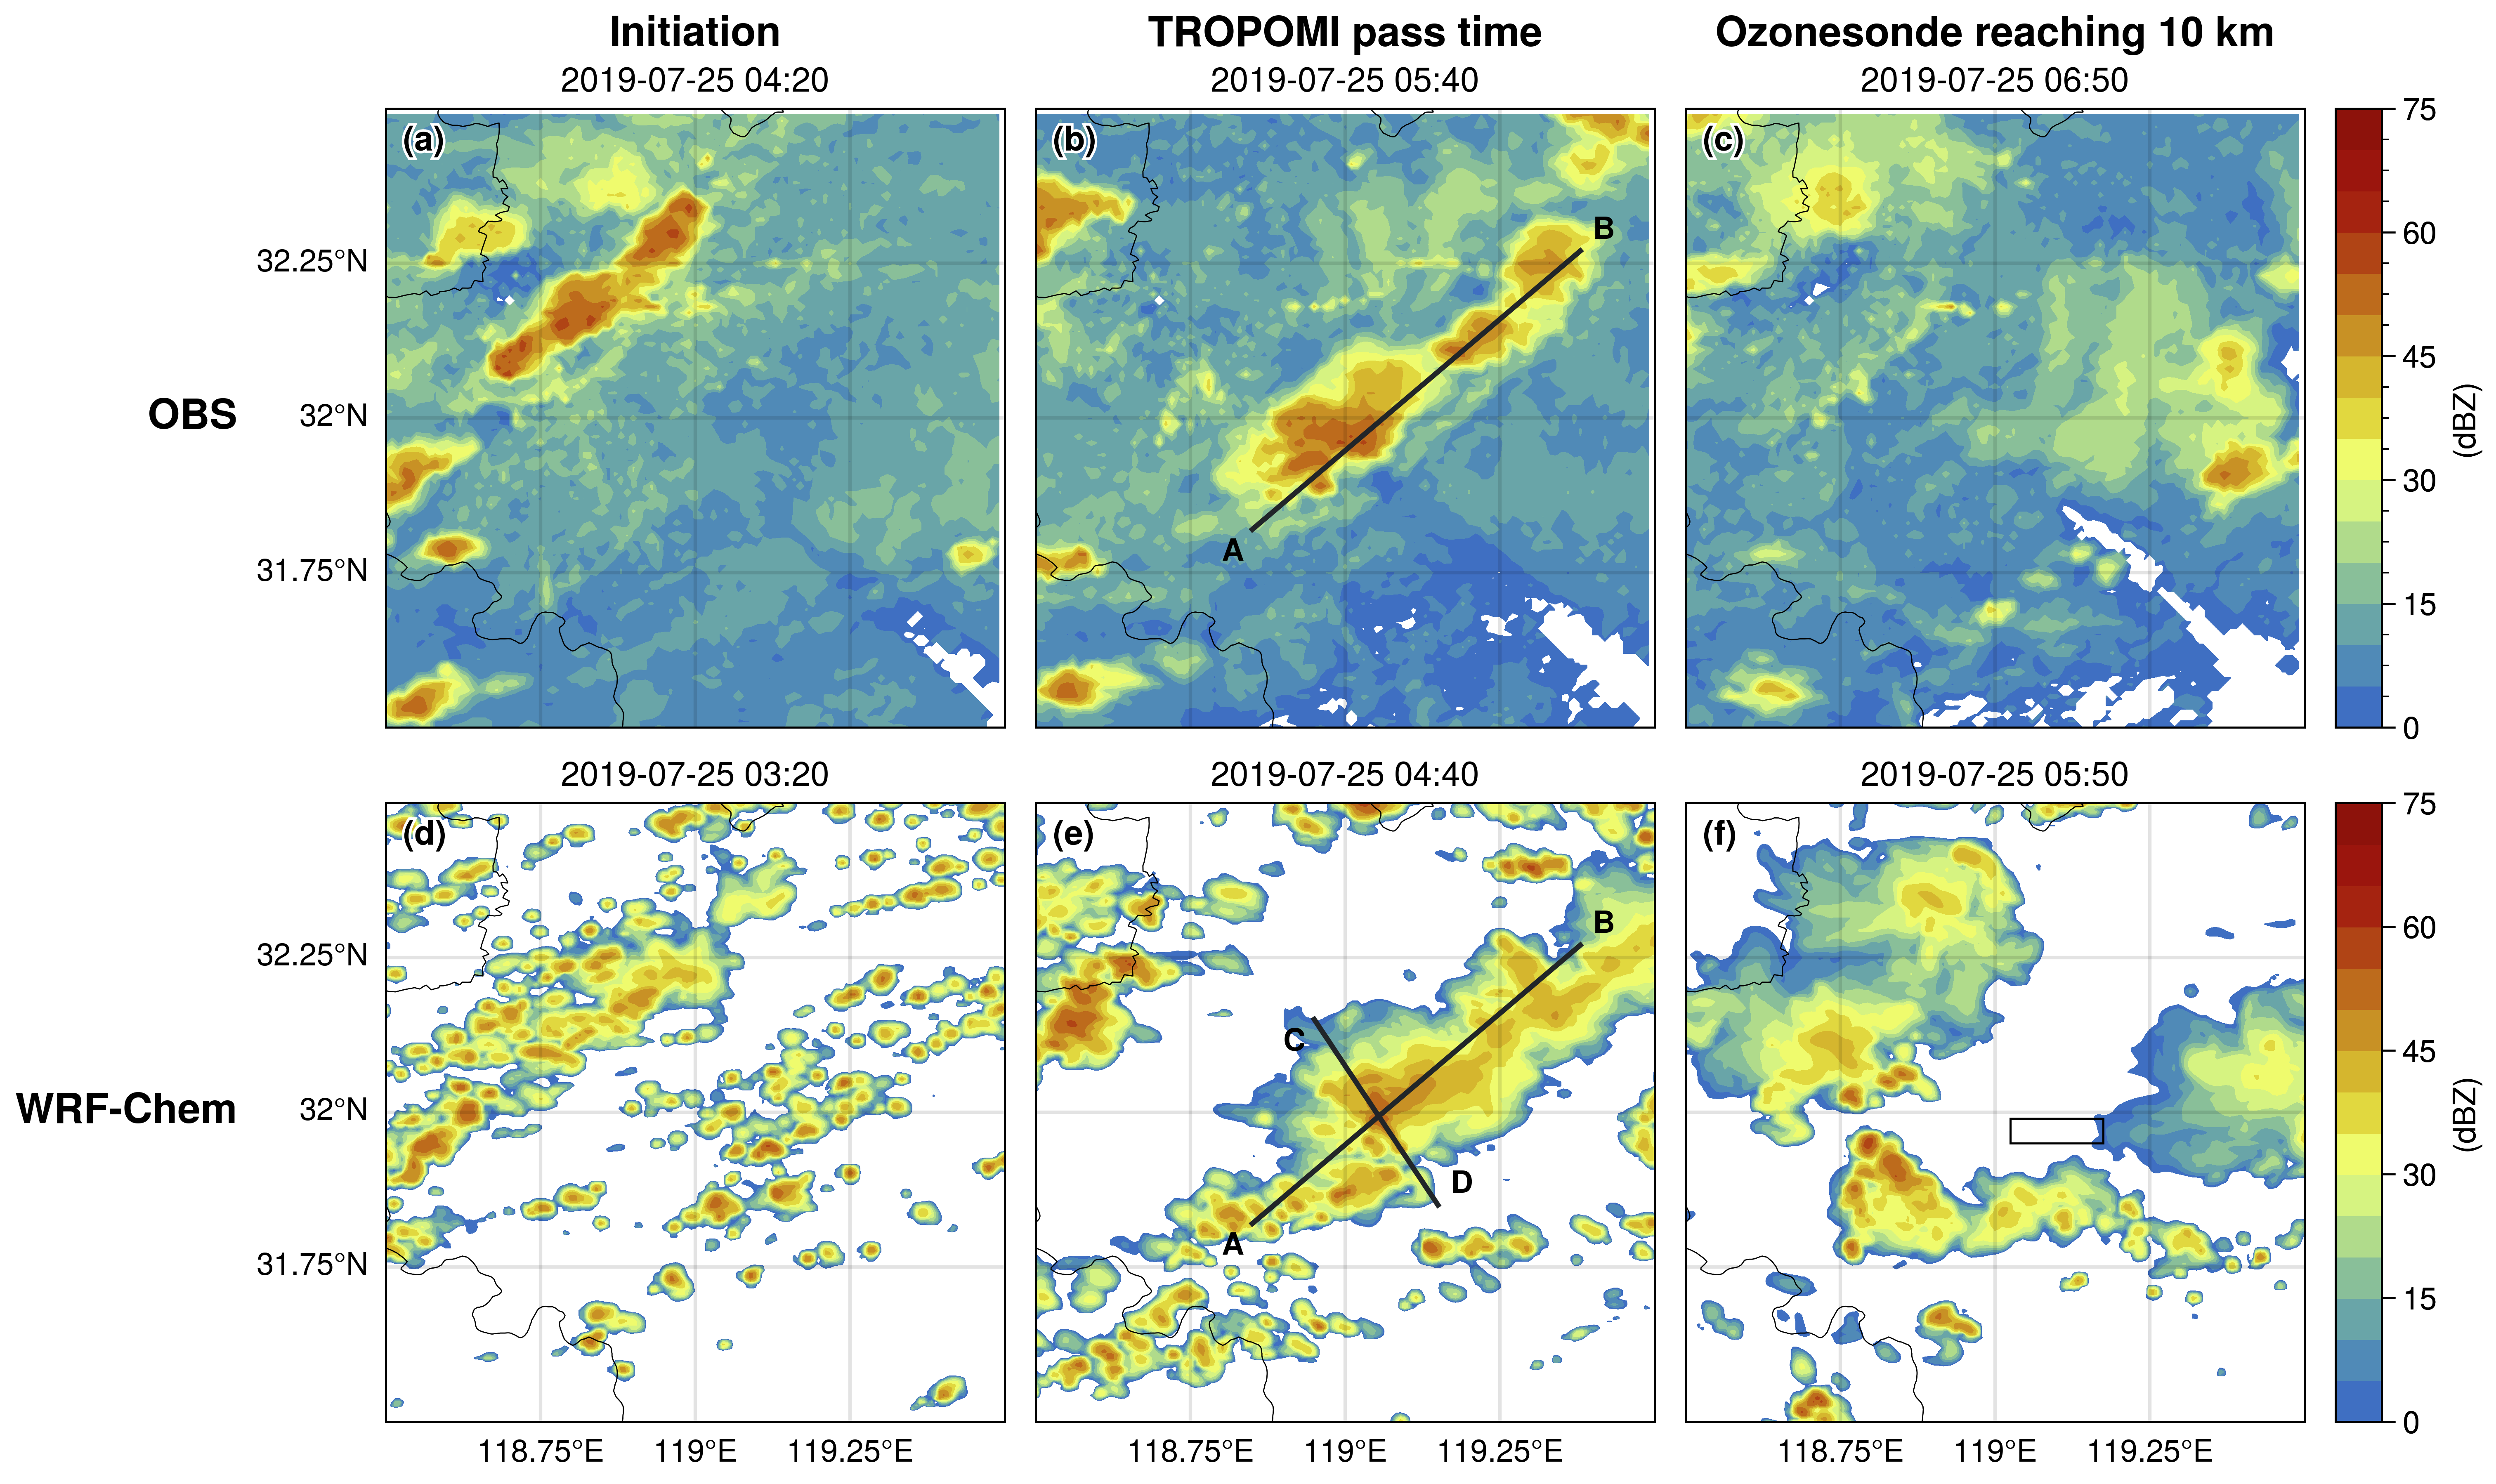
\includegraphics[width=0.9\textwidth]{./figures/comp_crf_2019.png}
\caption{在 (a) 04:20 UTC、(b) 05:40 UTC 和 (c) 06:50 UTC 观测到的雷达组合反射率。
         (d--e) WRF-Chem 在雷达观测时间前一小时模拟的雷达组合反射率。
         (b) 和 (e) 中的 AB 实线是图 \ref{fig:comp_dbzcross_2019} 的剖面线。
         (e)中的CD实线是图\ref{fig:tendency_o3}b的剖面线。
         黑色矩形是与臭氧探空仪进行比较的区域。\\
         Figure \ref{fig:comp_crf_2019}. Observed radar composite reflectivity at (a) 04:20 UTC, (b) 05:40 UTC, and (c) 06:50 UTC.
        (d--e) WRF-Chem simulated composite reflectivity one hour before the radar observation times.
        The AB solid lines in (b) and (e) are cross section lines for Fig. \ref{fig:comp_dbzcross_2019}.
        The CD solid line in (e) is the cross section line for Fig. \ref{fig:tendency_o3}b.
        The black rectangle is the region for the comparison with ozonesonde.}
\label{fig:comp_crf_2019}
\end{figure}

\begin{figure}[htbp]
\centering
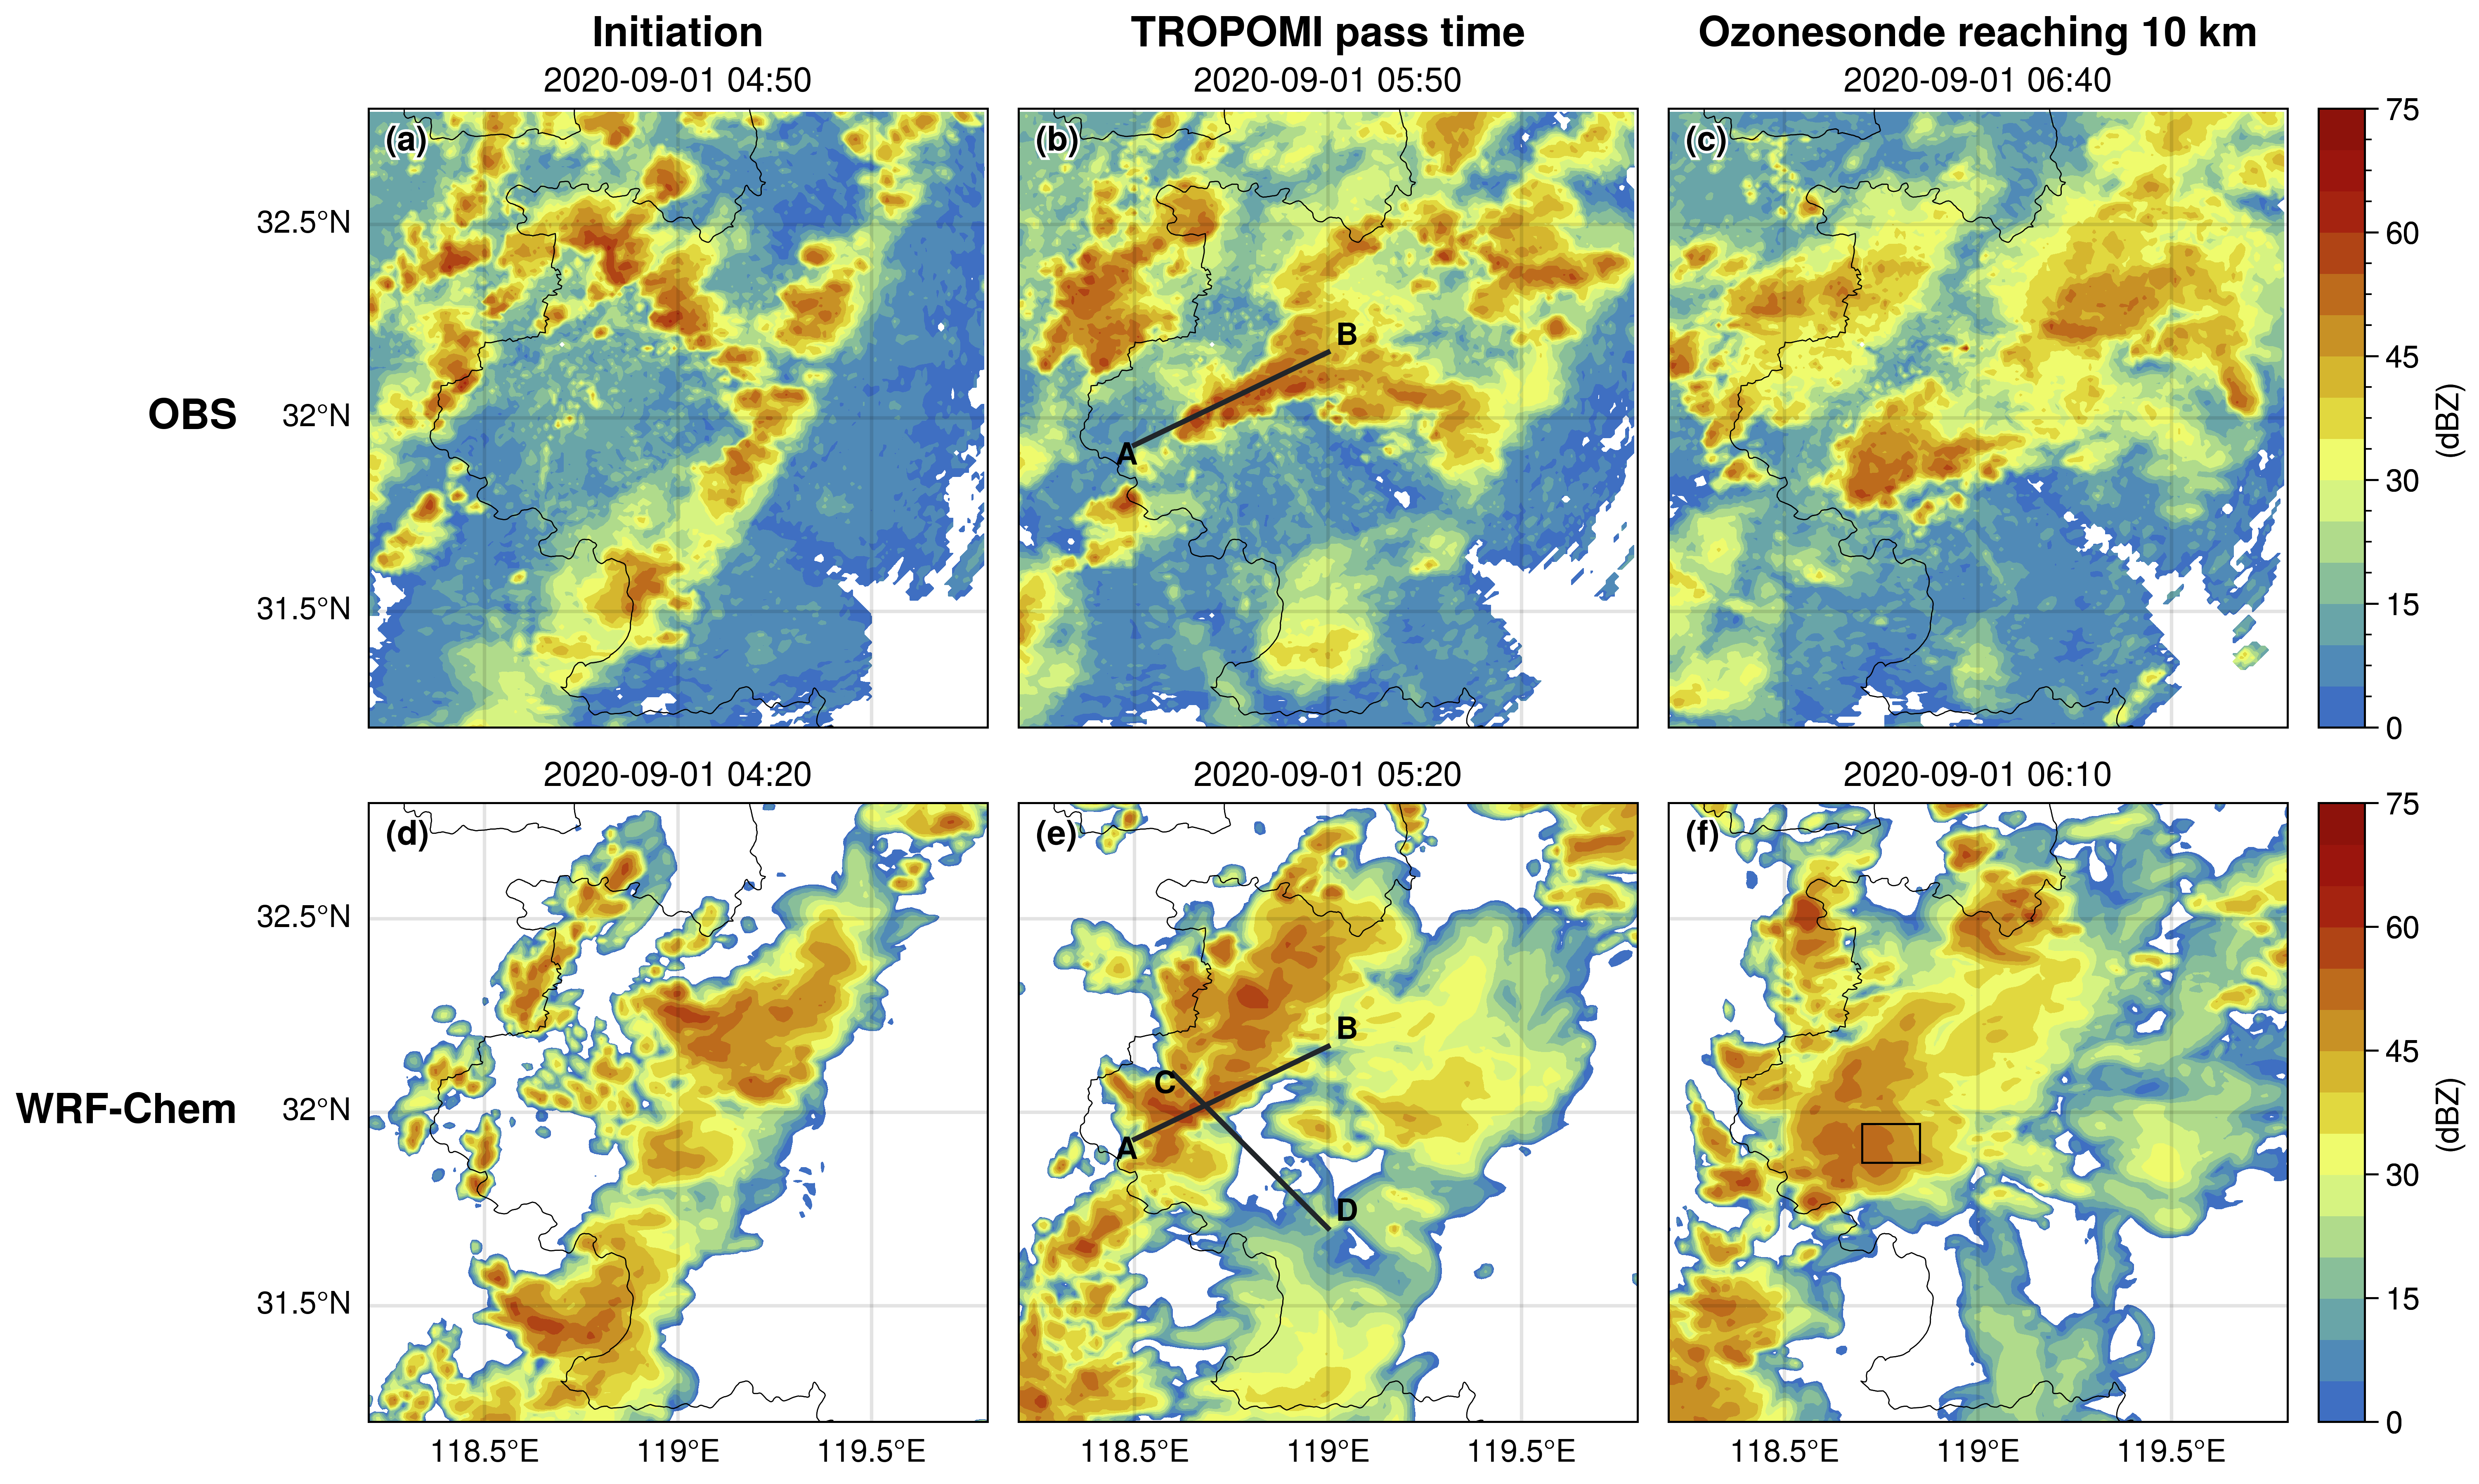
\includegraphics[width=0.9\textwidth]{./figures/comp_crf_2020.png}
\caption{与图\ref{fig:comp_crf_2019} 相同,但针对2020年9月1日的对流个例,模拟时间比雷达观测提前30分钟。\\
Figure \ref{fig:comp_crf_2020}. Same as Fig. \ref{fig:comp_crf_2019} but for the case on 01 September 2020.
The simulation time is 30 minutes ahead of each radar observation.}
\label{fig:comp_crf_2020}
\end{figure}

\begin{figure}[htbp]
\centering
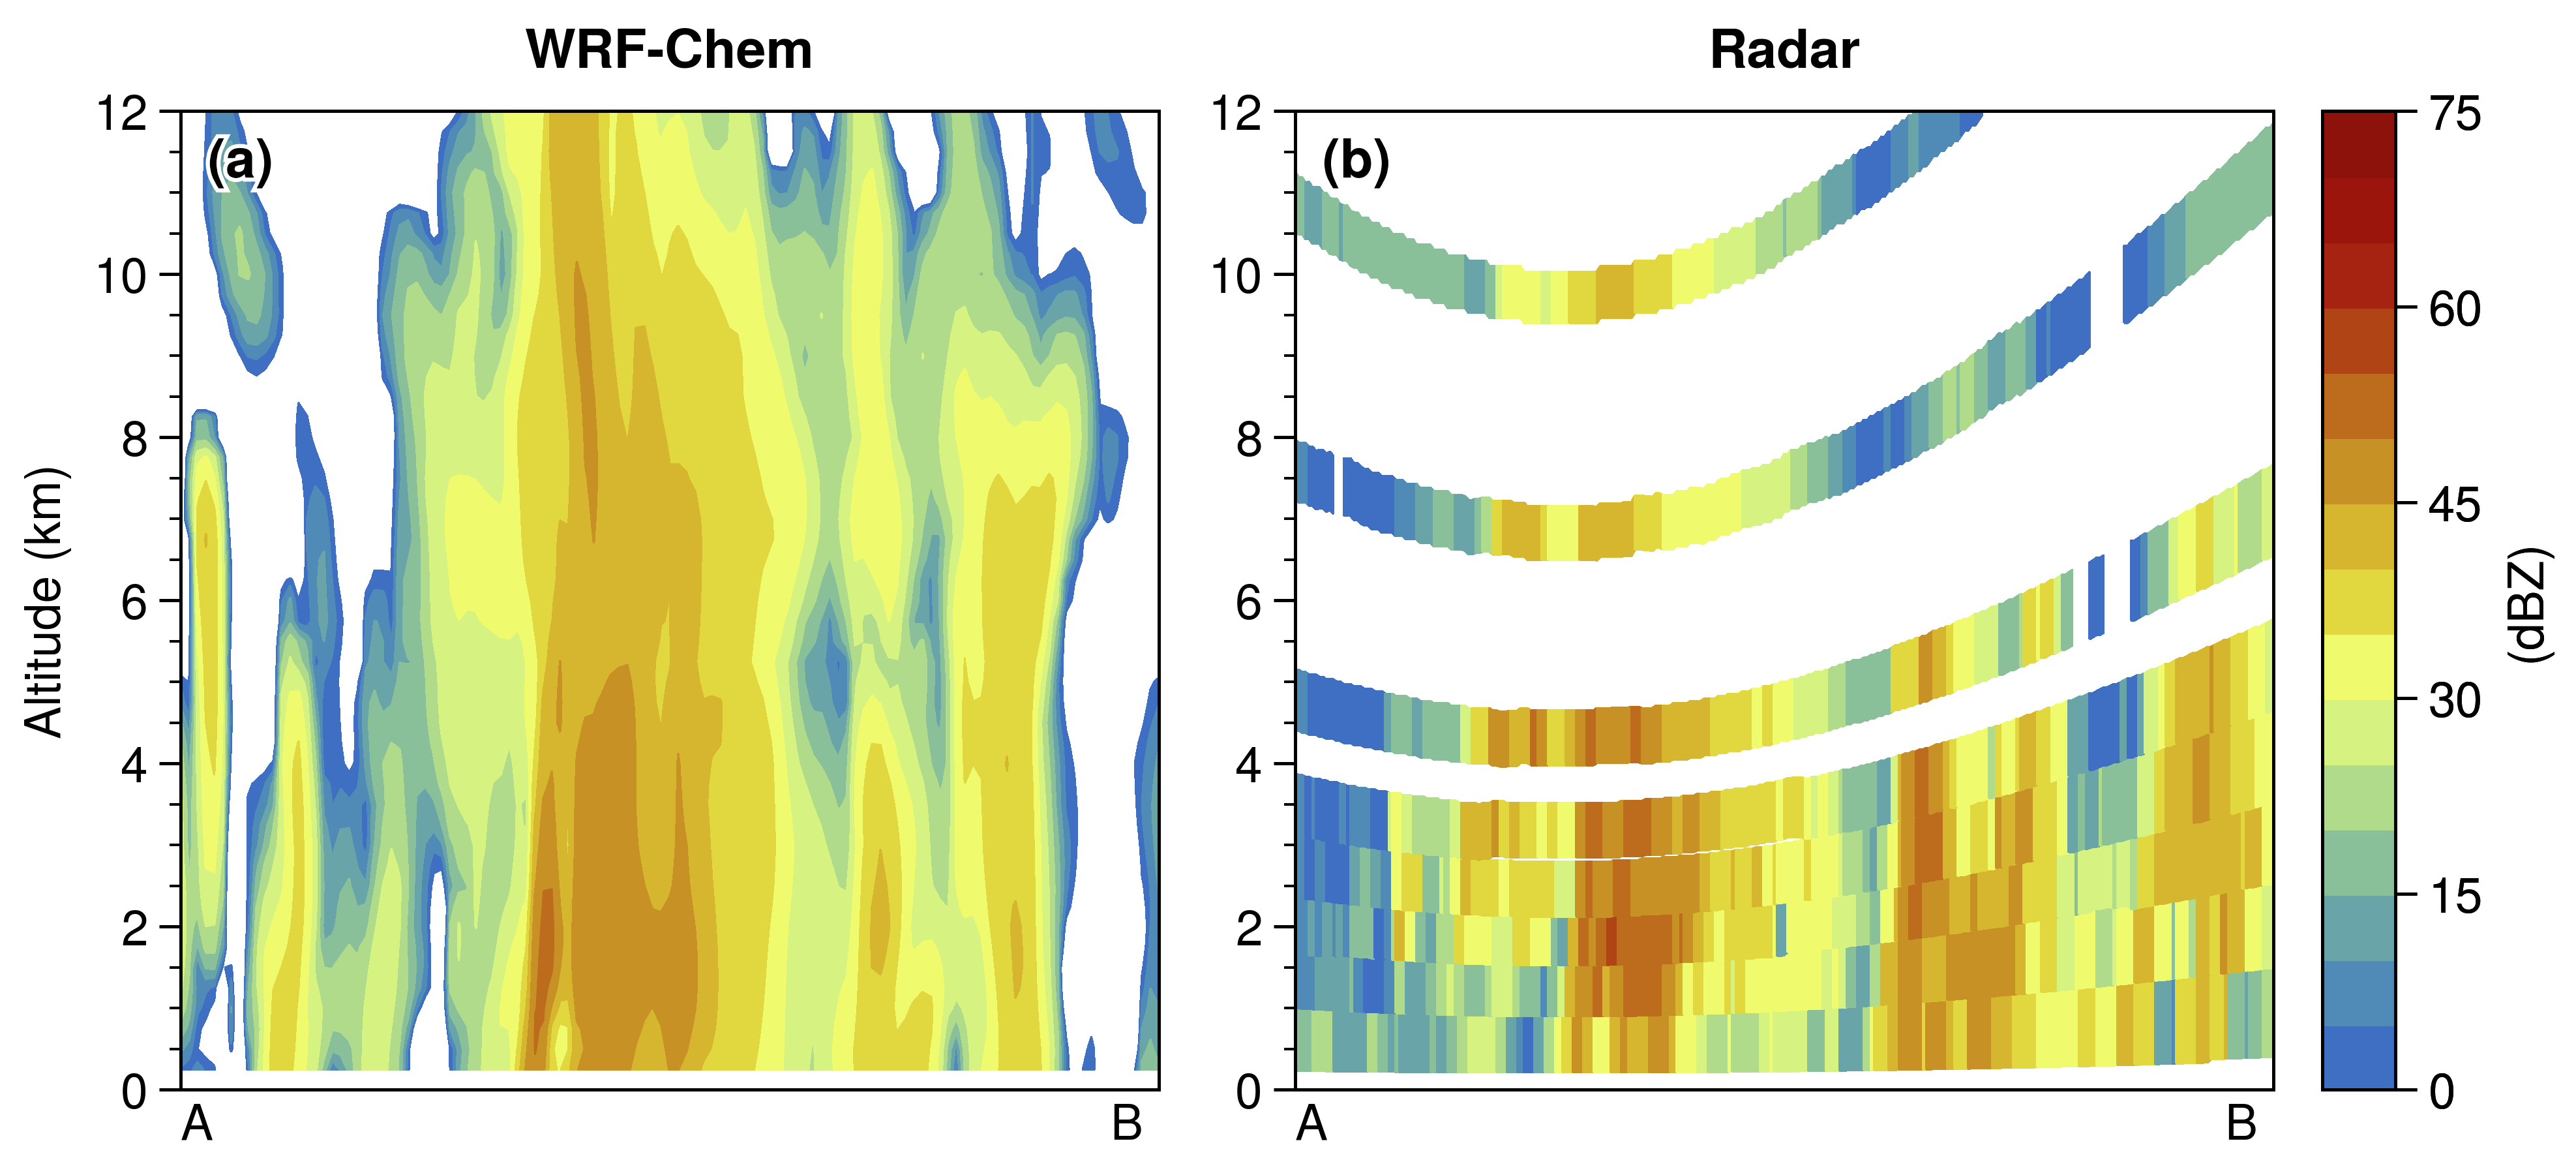
\includegraphics[width=0.8\textwidth]{./figures/comp_dbzcross_2019.png}
\caption{沿着图\ref{fig:comp_crf_2019}中AB线剖得的2019年7月25日(a)WRF-Chem模拟的和(b)雷达观测的雷达反射率。\\
Figure \ref{fig:comp_dbzcross_2019}. Vertical cross sections of (a) WRF-Chem simulated and (b) observed radar reflectivity fields along the transect lines (AB) in Fig. \ref{fig:comp_crf_2019} for 25 July, 2019.}
\label{fig:comp_dbzcross_2019}
\end{figure}

\begin{figure}[htbp]
\centering
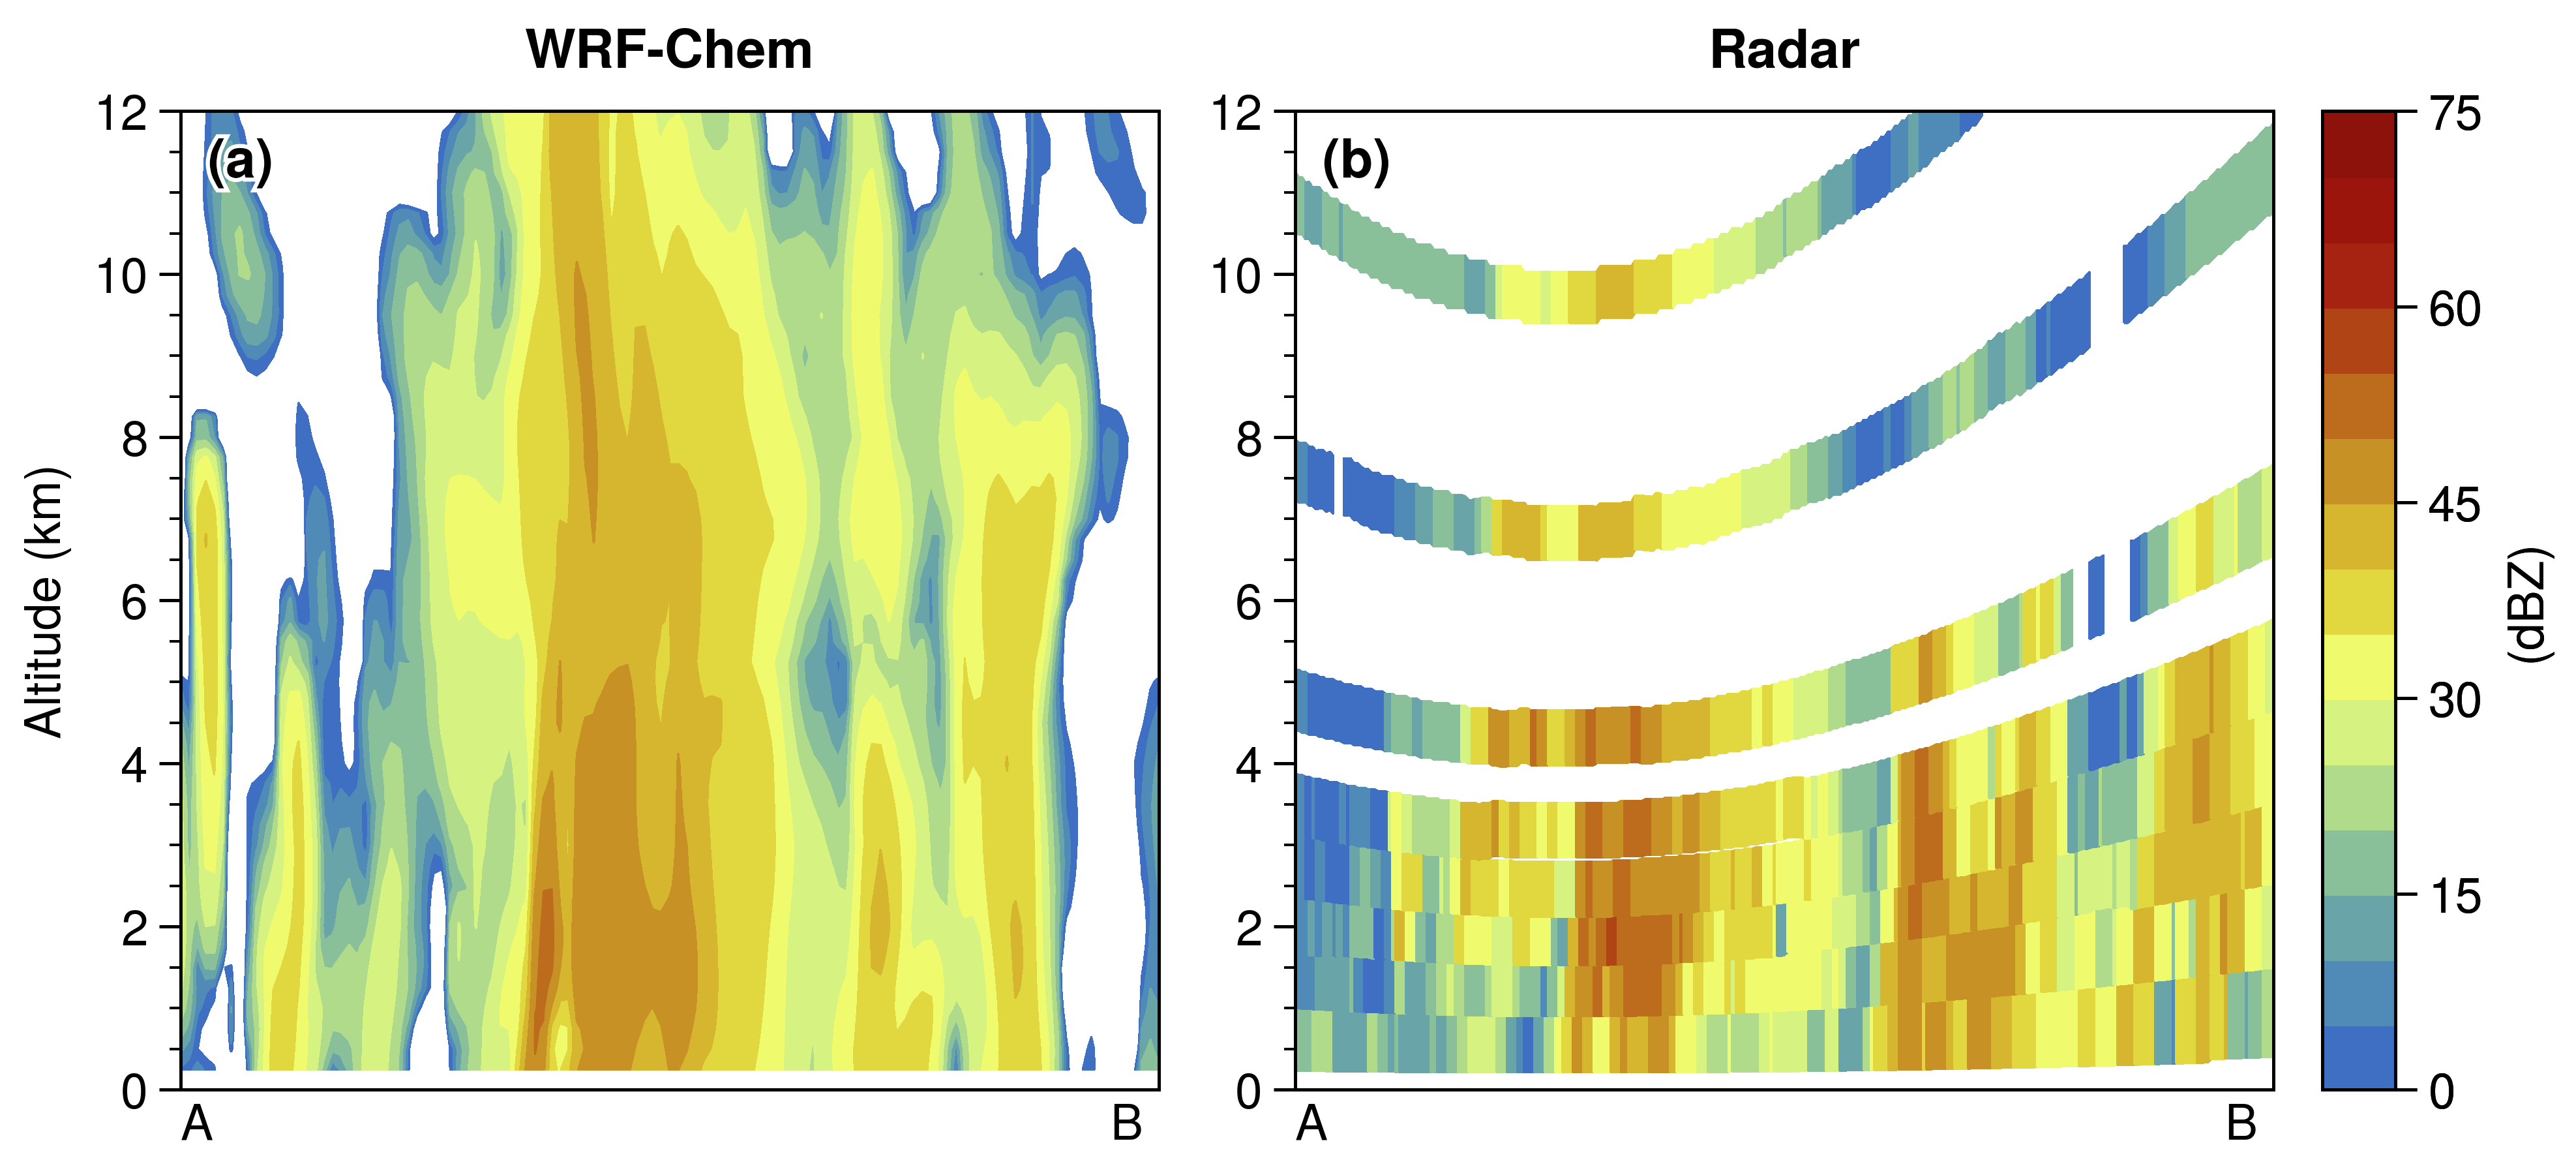
\includegraphics[width=0.8\textwidth]{./figures/comp_dbzcross_2019.png}
\caption{与图\ref{fig:comp_dbzcross_2019}相同,但针对2020年9月1日的对流个例。\\
Figure \ref{fig:comp_dbzcross_2020}. Same as Figure \ref{fig:comp_dbzcross_2019} but for the case on 01 September 2020.}
\label{fig:comp_dbzcross_2020}
\end{figure}


\begin{figure}[htbp]
\centering
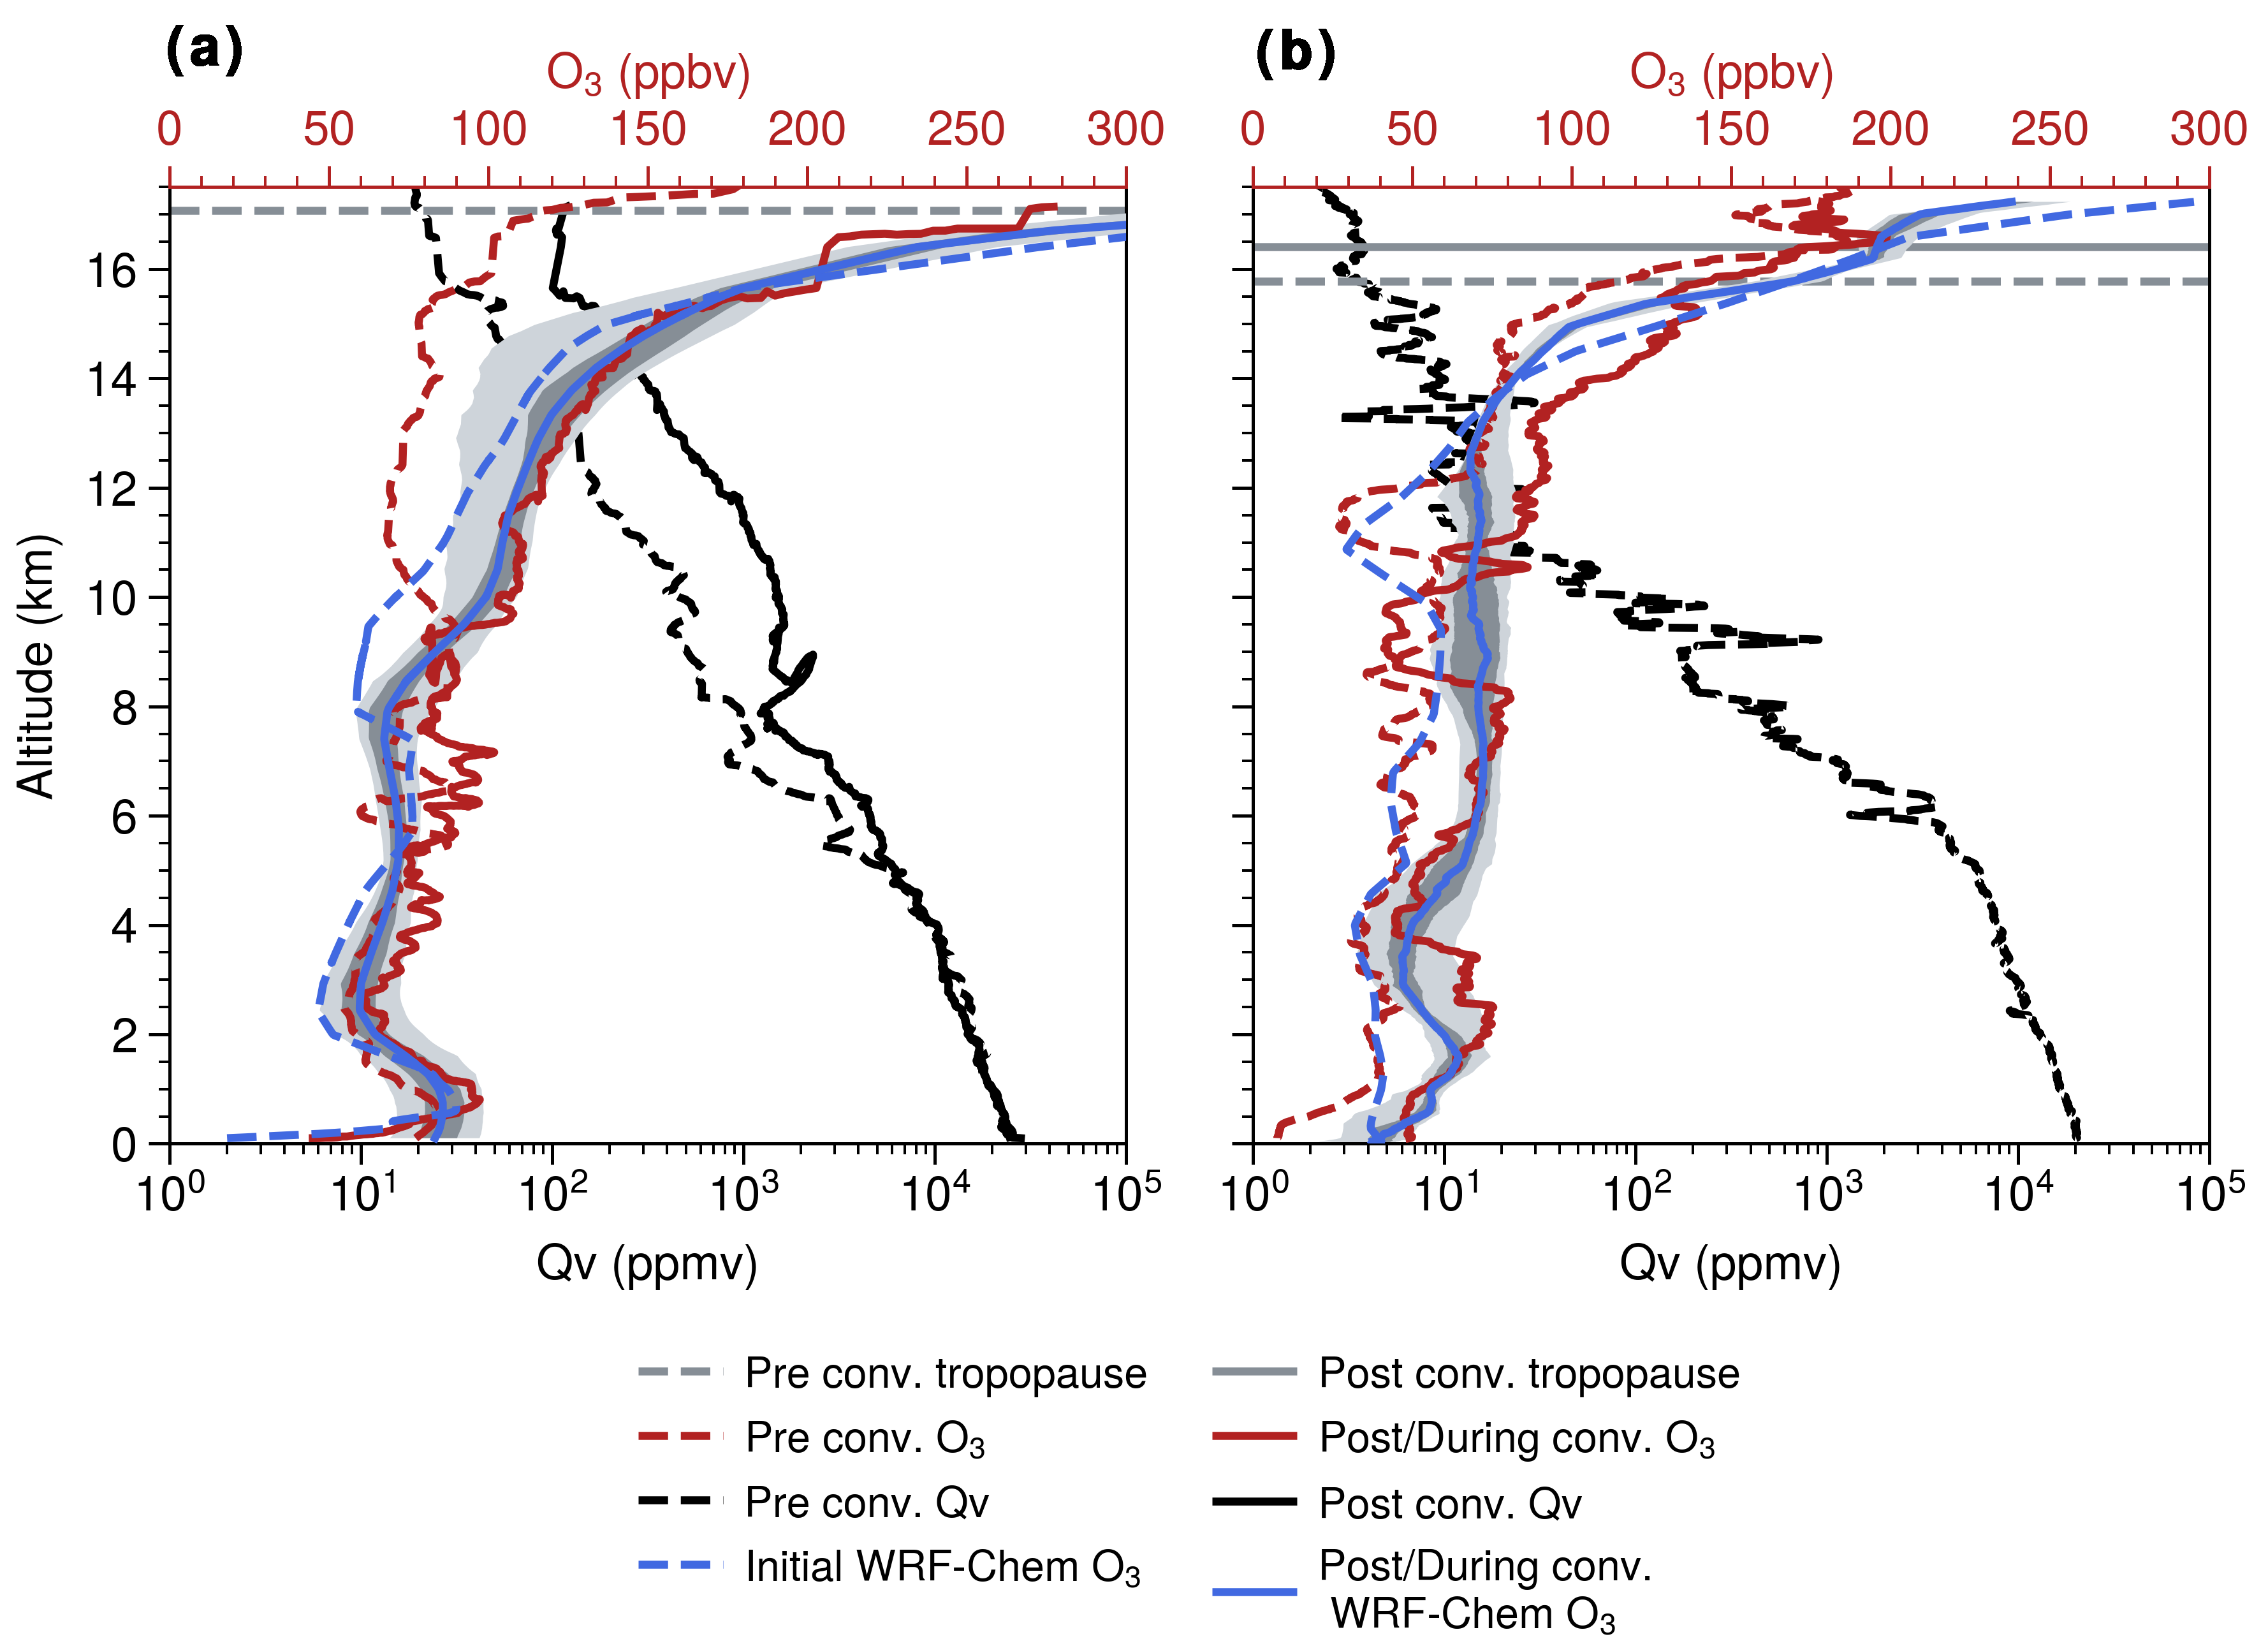
\includegraphics[width=0.8\textwidth]{./figures/ozonesonde_profile.png}
\caption{对流前(虚线)和对流后/对流期间(实线)探空观测到的O$_3$(红色)和Q$_v$(黑色)廓线。
模式初始(虚线)和对流后或对流期间(实线)的O$_3$廓线为蓝色。
深灰色阴影是50\%的置信区间,浅色是90\%的置信区间,灰线是第一对流层顶。\\
Figure \ref{fig:ozonesonde_profile}. Observed O$_3$ (red) and Qv (black) profiles in the pre-convection (dashed) and post-convection/during-convection (solid) periods.
The initial (dashed) and simulated post-convection or during-convection (solid) O$_3$ profiles are in blue.
The dark gray shading is the 50 \% confidence interval while the light one is the 90 \% confidence interval.
The gray lines are the lapse rate tropopauses.
}
\label{fig:ozonesonde_profile}
\end{figure}




\section{结果与讨论}

\subsection{动力输送和化学反应对臭氧变化的贡献} \label{subsect:convec_impacts}

为了探究对流后上对流层O$_3$浓度增大的原因,我们分为三个阶段(初生、发展和消散)分析了臭氧探空仪所经区域中O$_3$平均浓度的垂直廓线(图\ref{fig:tendency_o3}a 和 d)。
其中,2020年个例的上对流层O$_3$在整个周期内一直在增加,而2019年的个例由于发展阶段低浓度O$_3$空气的抬升,O$_3$浓度降低,接着又开始增大,这种现象可以用发展阶段的O$_3$垂直剖面来解释(图\ref{fig:tendency_o3}b和e)。
在2019年的个例中,低O$_3$浓度的空气块通过上升气流达到16 km,然后对流后方的高O$_3$浓度空气被夹卷进该区域。
而2020年个例中观测到增加的O$_3$,主要来自垂直传输的背景O$_3$浓度。

为了确定两种影响之间的差异,我们分析了对流期间10--14 km的平均累计物理变化速率 (IPR,图\ref{fig:tendency_o3}c和f)。
一般来说,水平平流 (advh) 和垂直平流 (advz) 的相反趋势支配着2019年上对流层O$_3$产率的净下降。
其中强上升气流使得低O$_3$浓度的空气块得以抬升,故垂直平流(advz)的贡献在10--11.5 km之间为负,而在11.5到13.8km 之间为正,即存在向下输送的高浓度O$_3$。
此外,由于2020年对流个例发生后的Q$_v$较高(图\ref{fig:ozonesonde_profile}a)且对流层顶高于云区(图\ref{fig:tendency_o3}b),
所以其上升气流不足以像中尺度对流系统一样将平流层高浓度的O$_3$挟至对流层\citep{Phoenix.2020}。
虽然动力输送在O$_3$的变化中起着重要作用,但不能忽视正的化学贡献,尤其是2020年对流期间上对流层O$_3$的净增加。
具体来说,在两次个例中化学反应对O$_3$起到了正贡献,其影响程度是动力输送的5--10倍,这表明化学贡献在对流的整个生命期中占主导地位。


\begin{figure}[htbp]
\centering
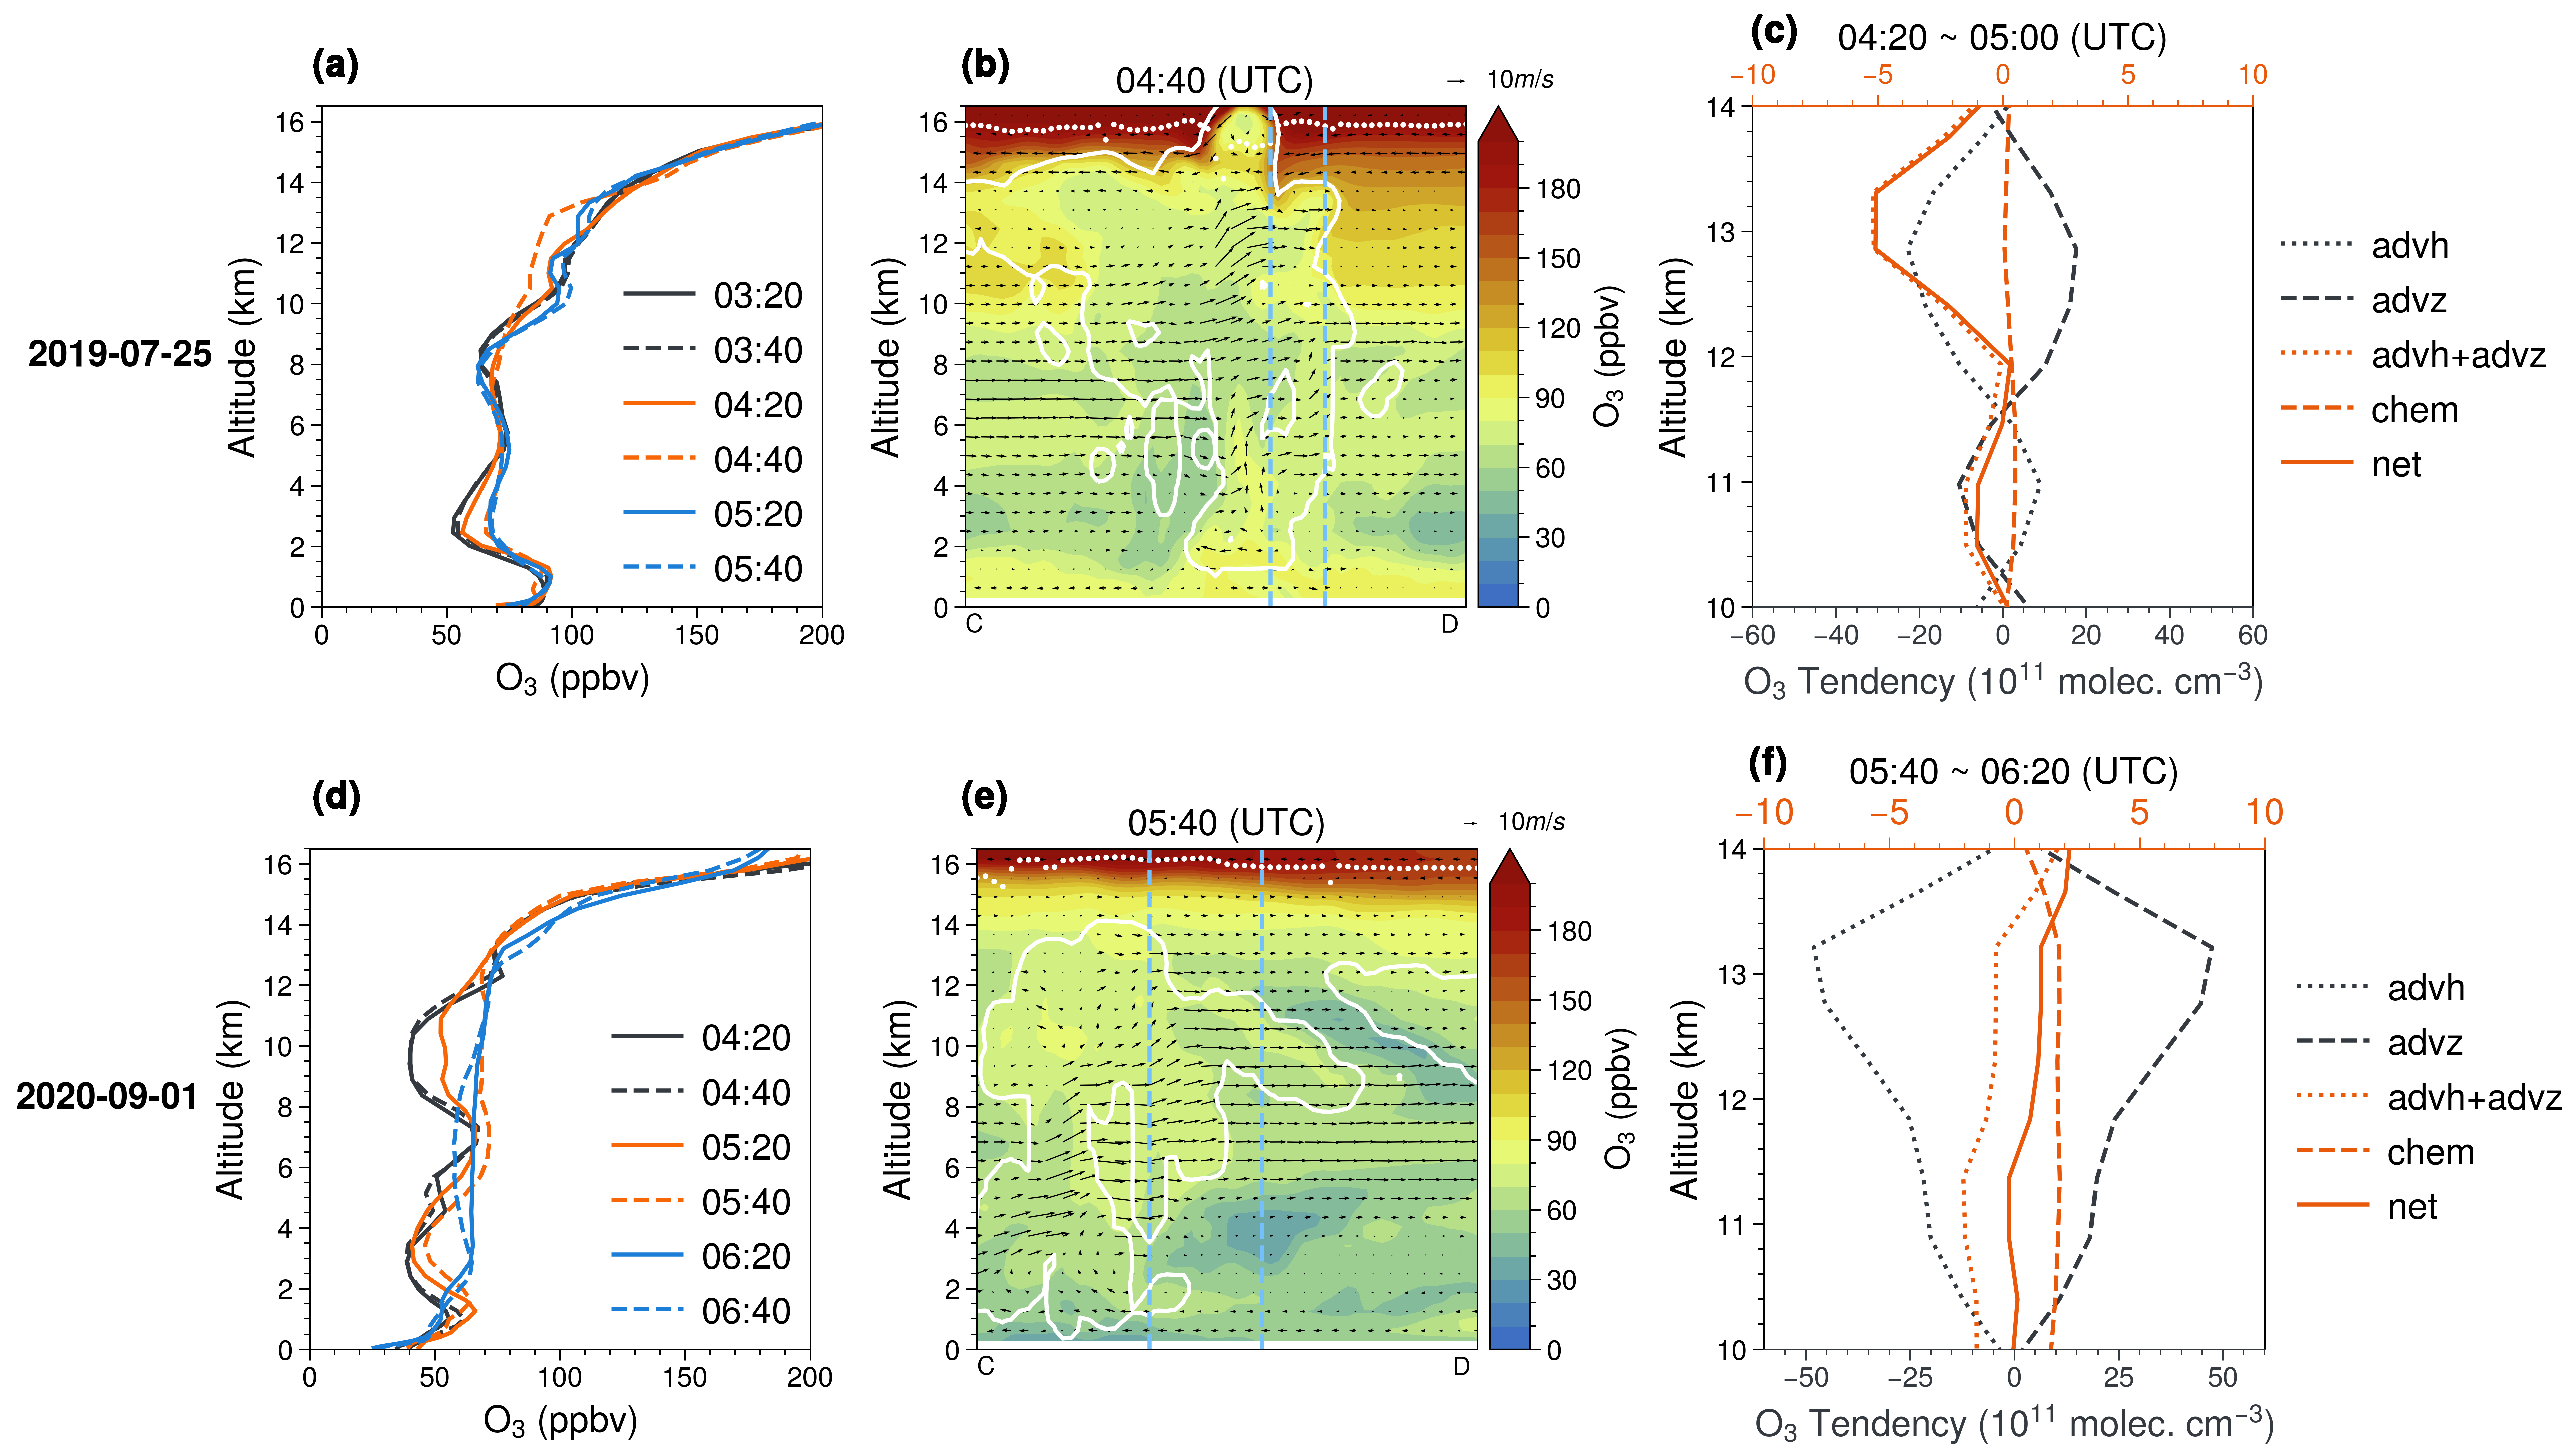
\includegraphics[width=\textwidth]{./figures/tendency_o3.png}
\caption{
(a, d) 臭氧探空仪经过区域的O$_3$平均浓度剖面,包括三个阶段:初生(黑色)、发展(橙色)和消散(蓝色)。
(b,e)对流旺盛期内沿穿过对流核心(图 \ref{fig:comp_crf_2019}e 和图 \ref{fig:comp_crf_2020}f)的O$_3$剖面。
蓝色虚线代表臭氧探空仪经过区域的边界,第一对流层顶显示为白点。
白线为云边界(云液态水混合比[q$_{cloud}$]和冰混合比[q$_{ice}$]之和 $\geq$ 0.01 g/kg)。
(c, f) 对流旺盛期的水平平流 (advh)、垂直平流 (advz) 和化学贡献 (chem)引起的O$_3$净生产率和趋势的垂直分布。
\\
Figure \ref{fig:tendency_o3}. (a, d) The mean O$_3$ profiles in the regions passed by the ozonesondes
at three stages: initiation (black), development (orange), and dissipation (blue).
(b, e) Vertical O$_3$ distribution within the convective periods along the line crossing the convective core (Fig. \ref{fig:comp_crf_2019}e and Fig. \ref{fig:comp_crf_2020}f).
The blue dashed lines stand for the boundaries of regions passed by the ozonesondes, and the lapse rate tropopause is shown as the white dots.
The cloud boundaries (the sum of cloud liquid water mixing ratio [q$_{cloud}$] and ice mixing ratio [q$_{ice}$] $\geq$ 0.01 g/kg) are shown in white lines.
(c, f) The vertical distributions of the O$_3$ net production rate and tendency due to horizontal advection (advh), vertical (advz) advection, and chemistry (chem) during the convective periods.
}
\label{fig:tendency_o3}
\end{figure}


\subsection{闪电氮氧化物对臭氧的影响}

我们将开启和不开启LNO排放所得到的O$_3$累计物理变化速率进行对比,从而得到LNO$_x$对O$_3$的影响(表1)。
在2019年个例的对流旺盛期和整个生命周期中,LNO$_x$使得O$_3$的净产量降低了25\%。
对于2020年个例,由于站点附近闪电密度较小,化学贡献导致的O$_3$浓度下降不显著($\leq$1\%)。
而前人研究表明,LNO$_x$在天的时间尺度范围内可提高下风向的O$_3$产量\citep{Pickering.1996,DeCaria.2005}。
因此,有必要准确估计LNO$_x$的产率(见第\ref{chapter:PE}章)。

\begin{table*}[h]
\centering
\caption{平均O$_3$累积趋势的过程分析(10--14 km)\\ Table \ref{table:ipr} Process analysis table for the mean O$_3$ integrated tendencies (10--14 km)}
\begin{tabular}{@{\extracolsep{\fill}} cccccc}
\hline
  Period           & Time             & LNO (mol/flash) & advh + advz$^*$       & chem$^*$              & net$^*$    \\
\hline
Life Cycle         & 2019-07-25       & 0               & -3.3 (-24.6 \%)        & 16.7 (124.6 \%)        & 13.4       \\
                   & (03:20--05:40)   & 500             & -2.3 (-28.8 \%)        & 10.3 (128.8 \%)        & 8.0        \\
\cline{2-6}
                   & 2020-09-01       & 0               & 3.4  (9.6 \%)          & 32.0 (90.4 \%)         & 35.4       \\
                   & (04:20--06:40)   & 500             & 4.4  (12.1 \%)         & 31.9 (87.8 \%)         & 36.3       \\
\hline
Convective Period   & 2019-07-25      & 0              & -19.6 (140.0 \%)       & 5.6 (-40.0 \%)         & -14.0      \\
                    & (04:20--05:00)  & 500            & -20.0 (114.3 \%)       & 2.5 (-14.3 \% )        & -17.5      \\
\cline{2-6}
                    & 2020-09-01      & 0              & -9.7  (-131.1 \%)      & 17.1 (231.1 \% )       & 7.4        \\
                    & (05:40--06:20)  & 500            & -10.1 (-148.5 \%)      & 16.9 (248.5 \% )       & 6.8        \\
\hline
\multicolumn{6}{l}{$^{*}$单位是 10$^{10}$ molec. cm$^{-3}$。百分比是每种贡献在净O$_3$变化中的比例。} \\
\multicolumn{6}{l}{$^{*}$The unit is 10$^{10}$ molec. cm$^{-3}$. The percentage is the proportion of each part in the net O$_3$ change.}
\end{tabular}
\label{table:ipr}
\end{table*}


此外,我们利用TROPOMI数据将对流分为三个区域:新生闪电区、闪电下风向和闪电老化区(详见第\ref{subsect:lnox_affects_tropomi}节和图\ref{fig:s5p_amf_diff})。
首先使用基于不同LNO产率的模拟结果,获得O$_3$差异($\Delta$O$_3$) 的廓线(图\ref{fig:irr_timeseries}(a--c))。
$\Delta$O$_3$在2--5 km之间大部分为正(< 1 ppbv),在5--12 km 之间为负,
这与\citet{Ott.2007}研究的个例结论不一致,他们得出在所有高度上的臭氧都产生净损失(< 4 ppbv)。
此外,较高的LNO产率(700 mol/闪电)与默认产率(500 mol /闪电)所得的结果相比,所有高度的O$_3$浓度降低了不到 1 ppbv,甚至导致闪电下风向2--5 km之间的$\Delta$O$_3$为负(图\ref{fig:irr_timeseries}b)。
由于LNO$_x$在8--10 km 之间达到峰值,O$_3$浓度也在此层降低(2.6 ppbv)最多。

接着,我们应用积分反应速率(IRR)来评估O$_3$变化的化学机制以及LNO对$\Delta$O$_3$的影响。
我们分两层来看该影响,因为800--500 hPa上$\Delta$O$_3$为正,500--200 hPa上$\Delta$O$_3$为负。
对流层O$_3$主要由五个反应速率项控制\citep{Pickering.1990}:

\begin{eqnarray}
  \frac{d}{dt}[\mathrm{O_3}] & = & k_1[\mathrm{NO}][\mathrm{HO_2}] + \sum_{i}  k_i[\mathrm{NO}][\mathrm{R_iO_2}] \nonumber \\
                             && - k_3[\mathrm{H_2O}][\mathrm{O(^1D)}] - k_4[\mathrm{HO_2}][\mathrm{O_3}] - k_5[\mathrm{OH}][\mathrm{O_3}]
\end{eqnarray}

其中k$_i$是过氧自由基 (R$_i$O$_2$)与NO之间的反应速率系数。
每个反应对O$_3$贡献的时间序列如图\ref{fig:irr_timeseries}(d--i)所示。
总体而言,由于2019年个例的垂直运动更强(见第\ref{subsect:convec_impacts}节),故积分反应速率的时间序列变化更大,且所选两层的O$_3$总净化学产量保持正值。
具体而言,NO和HO$_2$之间的反应始终占主导地位,而RO$_2$对NO的氧化约占该产量的40\%--60\%。
O$_3$的主要损耗是光解反应(O(1D)和H$_2$O的反应),而O$_3$和OH之间的反应在对流期间与之相当。
O$_3$损耗的最低贡献,O$_3$ + HO$_2$ $\,\to\,$ OH + 2O$_2$,在对流旺盛期减少,因为LNO的产生捕获了本应与O$_3$反应的HO$_2$。
虽然LNO$_x$引起的总积分反应速率增加,在低层和高层分别为1.36$\cdot$10$^7$和2.60$\cdot$10$^6$ molec cm$^{-3}$ s$^{-1}$。
但是由于动力传输和与LNO$_x$化学贡献的综合作用,高层的O$_3$净产量实际上减少了(图\ref{fig:irr_timeseries}(a--c))。


\begin{figure}[h]
    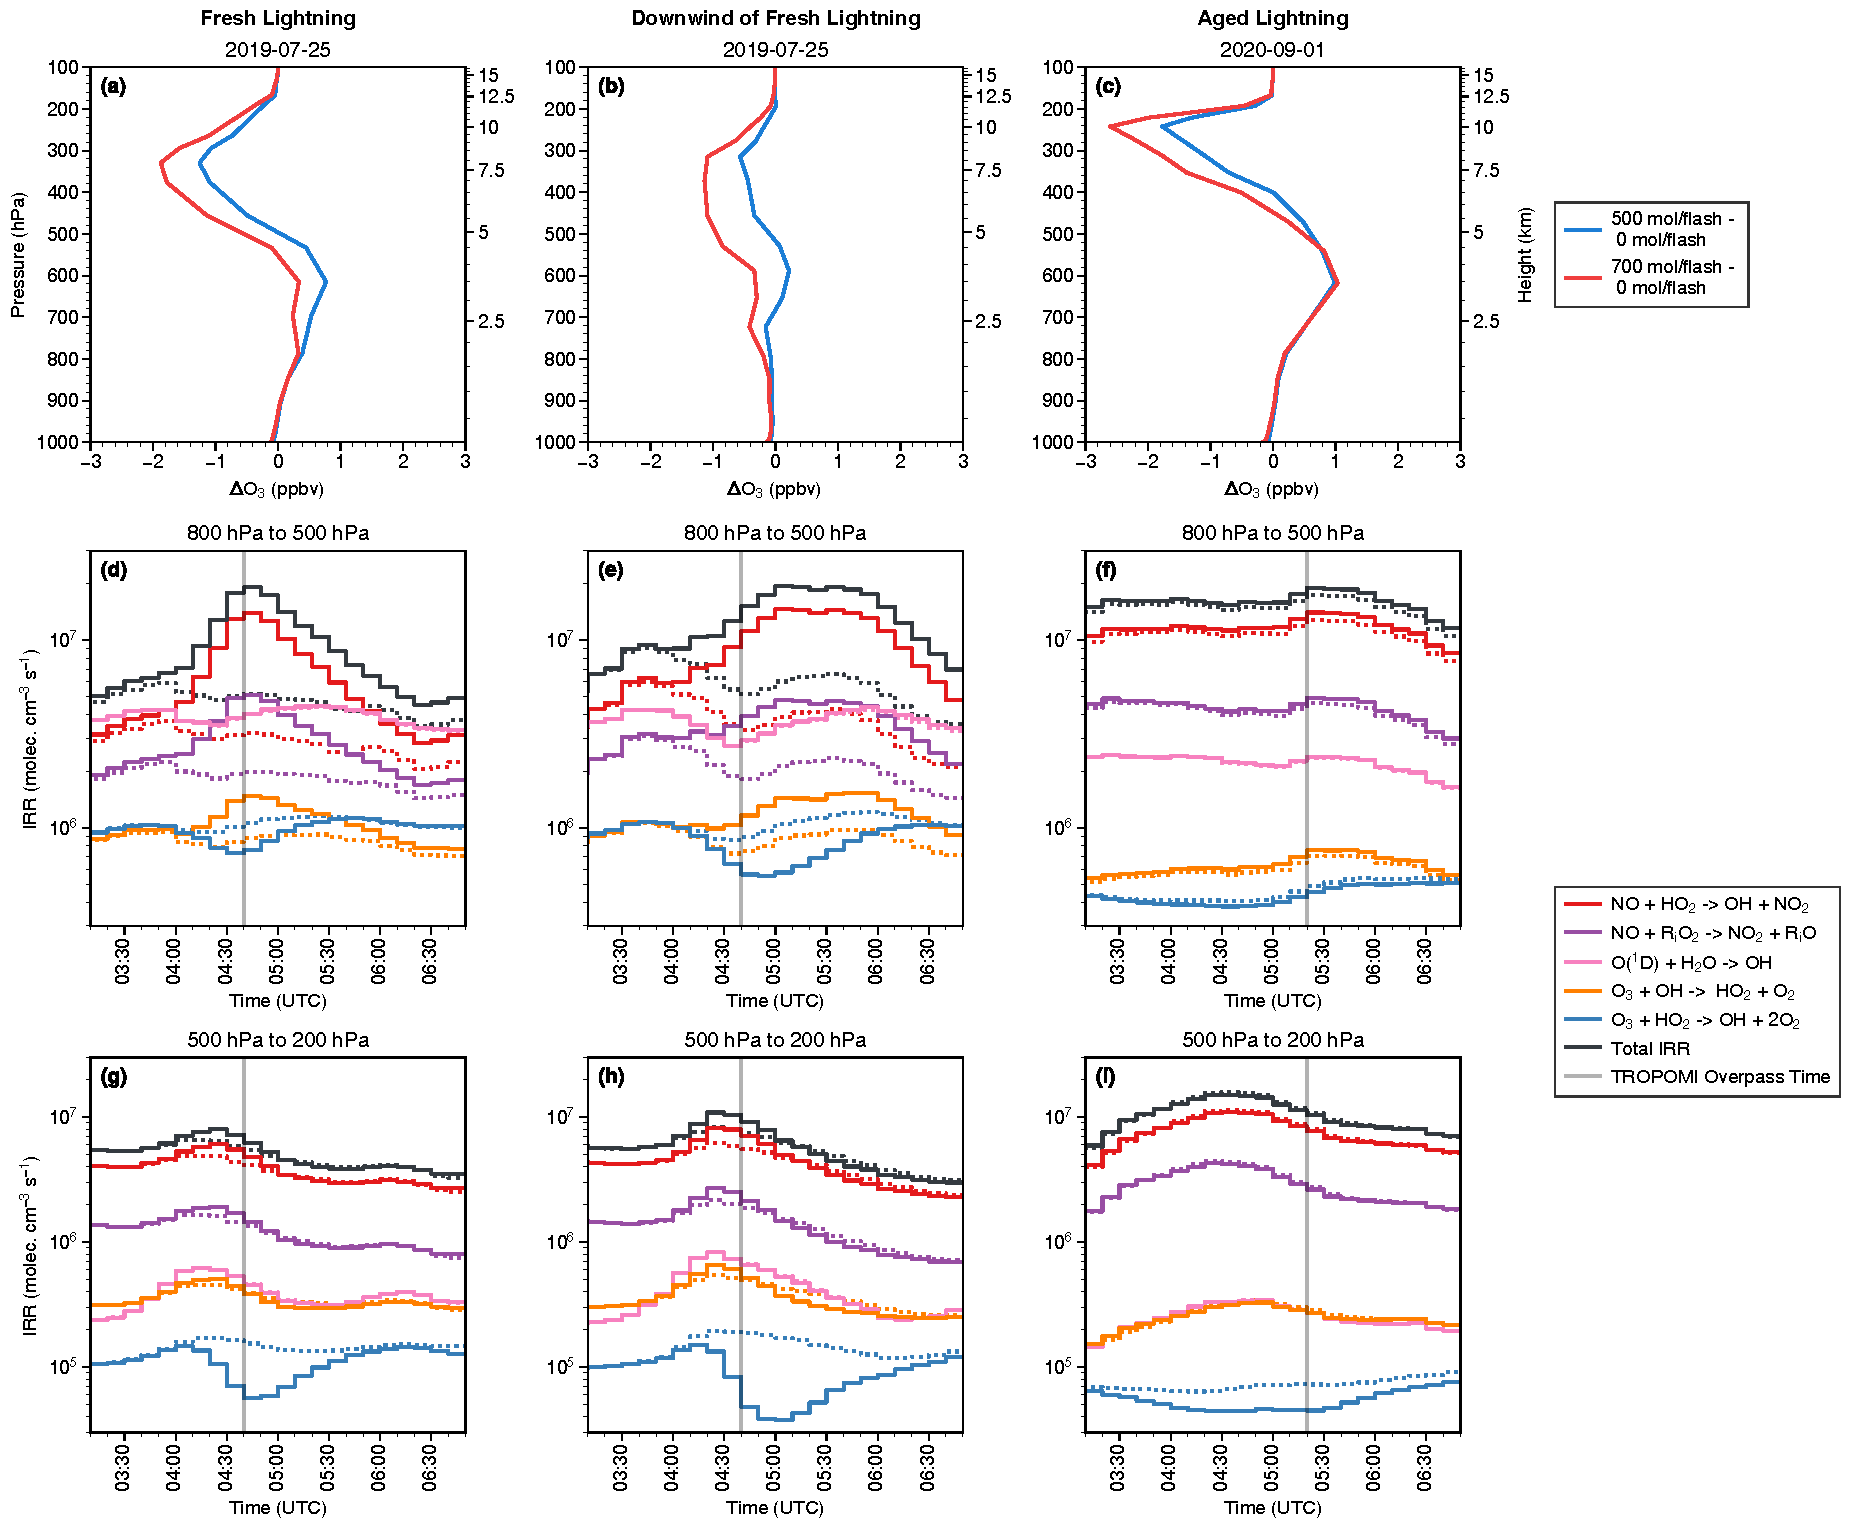
\includegraphics[width=16cm]{./figures/irr_timeseries.pdf}
    \caption{
    (a--c) 在图\ref{fig:s5p_amf_diff}定义的三个区域(新生闪电区、闪电下风向和闪电老化区)中,TROPOMI过境时由LNO$_x$所引起的O$_3$剖面变化。
    (d--f) 800 hPa 和 500 hPa 之间平均累积反应速率 (IRR) 的时间序列。其中图例显示了详细的物种和反应。总IRR是从生成O$_3$的IRR(红线和紫线)中减去O$_3$损失的IRR。
     实线为模拟中开启LNO (500 mol/flash)排放的IRR,而虚线表示没有LNO。
    (g--i) 与 (d--f) 相同,但在 500 hPa 和 200 hPa 之间。\\
    Figure \ref{fig:irr_timeseries}. (a--c) Changes in O$_3$ profiles due to LNO$_x$ at TROPOMI overpass time in three regions (fresh lightning region, downwind of fresh lightning, and aged lightning area) as defined in Fig. \ref{fig:s5p_amf_diff}.
    (d--f) Time series of the mean integrated reaction rate (IRR) between 800 hPa and 500 hPa.
    The legend shows detailed species and reactions.
    The Total IRR is the O$_3$ loss IRR subtracted from the O$_3$ production IRR (red and purple lines).
    The solid line shows the IRR with LNO (500 mol/flash) while the dashed line is without LNO.
    (g--i) Same as (d--f) but between 500 hPa and 200 hPa.
    }
    \label{fig:irr_timeseries}
\end{figure}



\subsection{闪电氮氧化物对反演产品的影响}  \label{subsect:lnox_affects_tropomi}


在利用卫星观测计算LNO$_x$产率之前,我们首先探讨了LNO$_x$对官方NO$_2$柱浓度产品的影响。
图\ref{fig:flash_scd}(a--d)将对流层NO$_2$斜柱浓度(S$_{\textrm{NO$_2$}}$)的分布与观测的闪电分布进行了比较。
尽管由于探测器饱和和光晕效应,闪电最活跃像素上的S$_{\textrm{NO$_2$}}$无效,但附近或对流出流区仍有有效数据。
在2019年的个例中,闪电发生在TROPOMI过境前不到30分钟,但2020年的个例中既有新生的也有老化的LNO$_2$(图\ref{fig:flash_scd}(d))。

具体而言,对流旺盛处((f$_r$) $\geq$ 0.7)的S$_{\textrm{NO$_2$}}$小于其他区域。
这与之前针对具有高闪电密度的大规模对流系统的研究结果相反\citep{Beirle.2009}。
导致这一差距的因素有四点:云顶高度、闪电次数、闪电发生时间和背景NO$_2$浓度。
由于TROPOMI只能探测到处于云层上方的LNO$_2$,因此当fr $\approx$ 1时,闪电次数不足或对流较弱都可能导致对流旺盛区的S$_{\textrm{NO$_2$}}$更小。
即如果f$_r$<1,则破碎或稀薄云层下方的污染NO$_2$则会部分被TROPOMI探测到。
而WRF-Chem的先验S$_{\textrm{NO$_2$}}$敏感性试验可以清楚地解释这种现象(图\ref{fig:s5p_apriori_scd})。
具有低f$_r$和高S$_{\textrm{NO$_2$}}$像素源自于背景 NO$_2$ 污染(图\ref{fig:s5p_apriori_scd}(a)和(e)),
但与没有LNO$_2$贡献的低S$_{\textrm{NO$_2$}}$相比,上对流层LNO$_2$增加的S$_{\textrm{NO$_2$}}$仍然可见(图\ref{fig:s5p_apriori_scd}(b)--d 和 (f)--(h))。

为了研究LNO$_x$对AMF$_\textrm{trop}$和AMF$_\textrm{LNO$_x$}$计算的重要性,我们将LNO产率的上限700 mol NO 每闪电\citep{Ott.2010}应用于WRF-Chem 。
接着我们通过独立替换三个对流层层中的NO$_2$廓线:对流层中层(MT,800 到 400 hPa)、对流层上层(UT,400 到 150 hPa)和整个对流层(地表到对流层顶)。
除非另有说明,否则后文AMF的变化是通过增加LNO$_x$获得的。
如图\ref{fig:s5p_amf_diff}显示,AMF变化主要由检测灵敏度高的上对流层LNO$_x$所控制\citep{Beirle.2009,Laughner.2017},且LNO$_x$产量在该高度达到峰值(图\ref{fig:nox_profile})。
虽然两种情况下AMF均降低了5\%--40\%,但AMF$_\textrm{trop}$的变化($\Delta$AMF$_\textrm{LNO$_x$}$)具有区域特异性。
可根据闪电活动对其进行分类:新生闪电区(MT ΔAMF\%)、闪电下风向(MT $\Delta$AMF$_\textrm{trop}$>20\%)和闪电老化区(UT $\Delta$AMF$_\textrm{trop}$>20\%)。
图\ref{fig:amf_contribution}(a)说明了云压(p$_{cloud}$)和f$_r$在这三个区域上的关系。
云层高于400 hPa(p$_{cloud}$< 400 hPa),新生闪电区的像素上f$_r$大于0.8,但闪电老化区和闪电下风向都有低于400 hPa的云层。
这与图\ref{fig:nox_profile}中的平均云压一致,并解释了为什么UT $\Delta$AMF$_\textrm{trop}$ > 20\% 在图\ref{fig:s5p_amf_diff}(b)i 和 (b)iii 中存在,这也正表明了在闪电老化区估算LNO$_x$的可能性。


\begin{figure}[h]
    \centering
    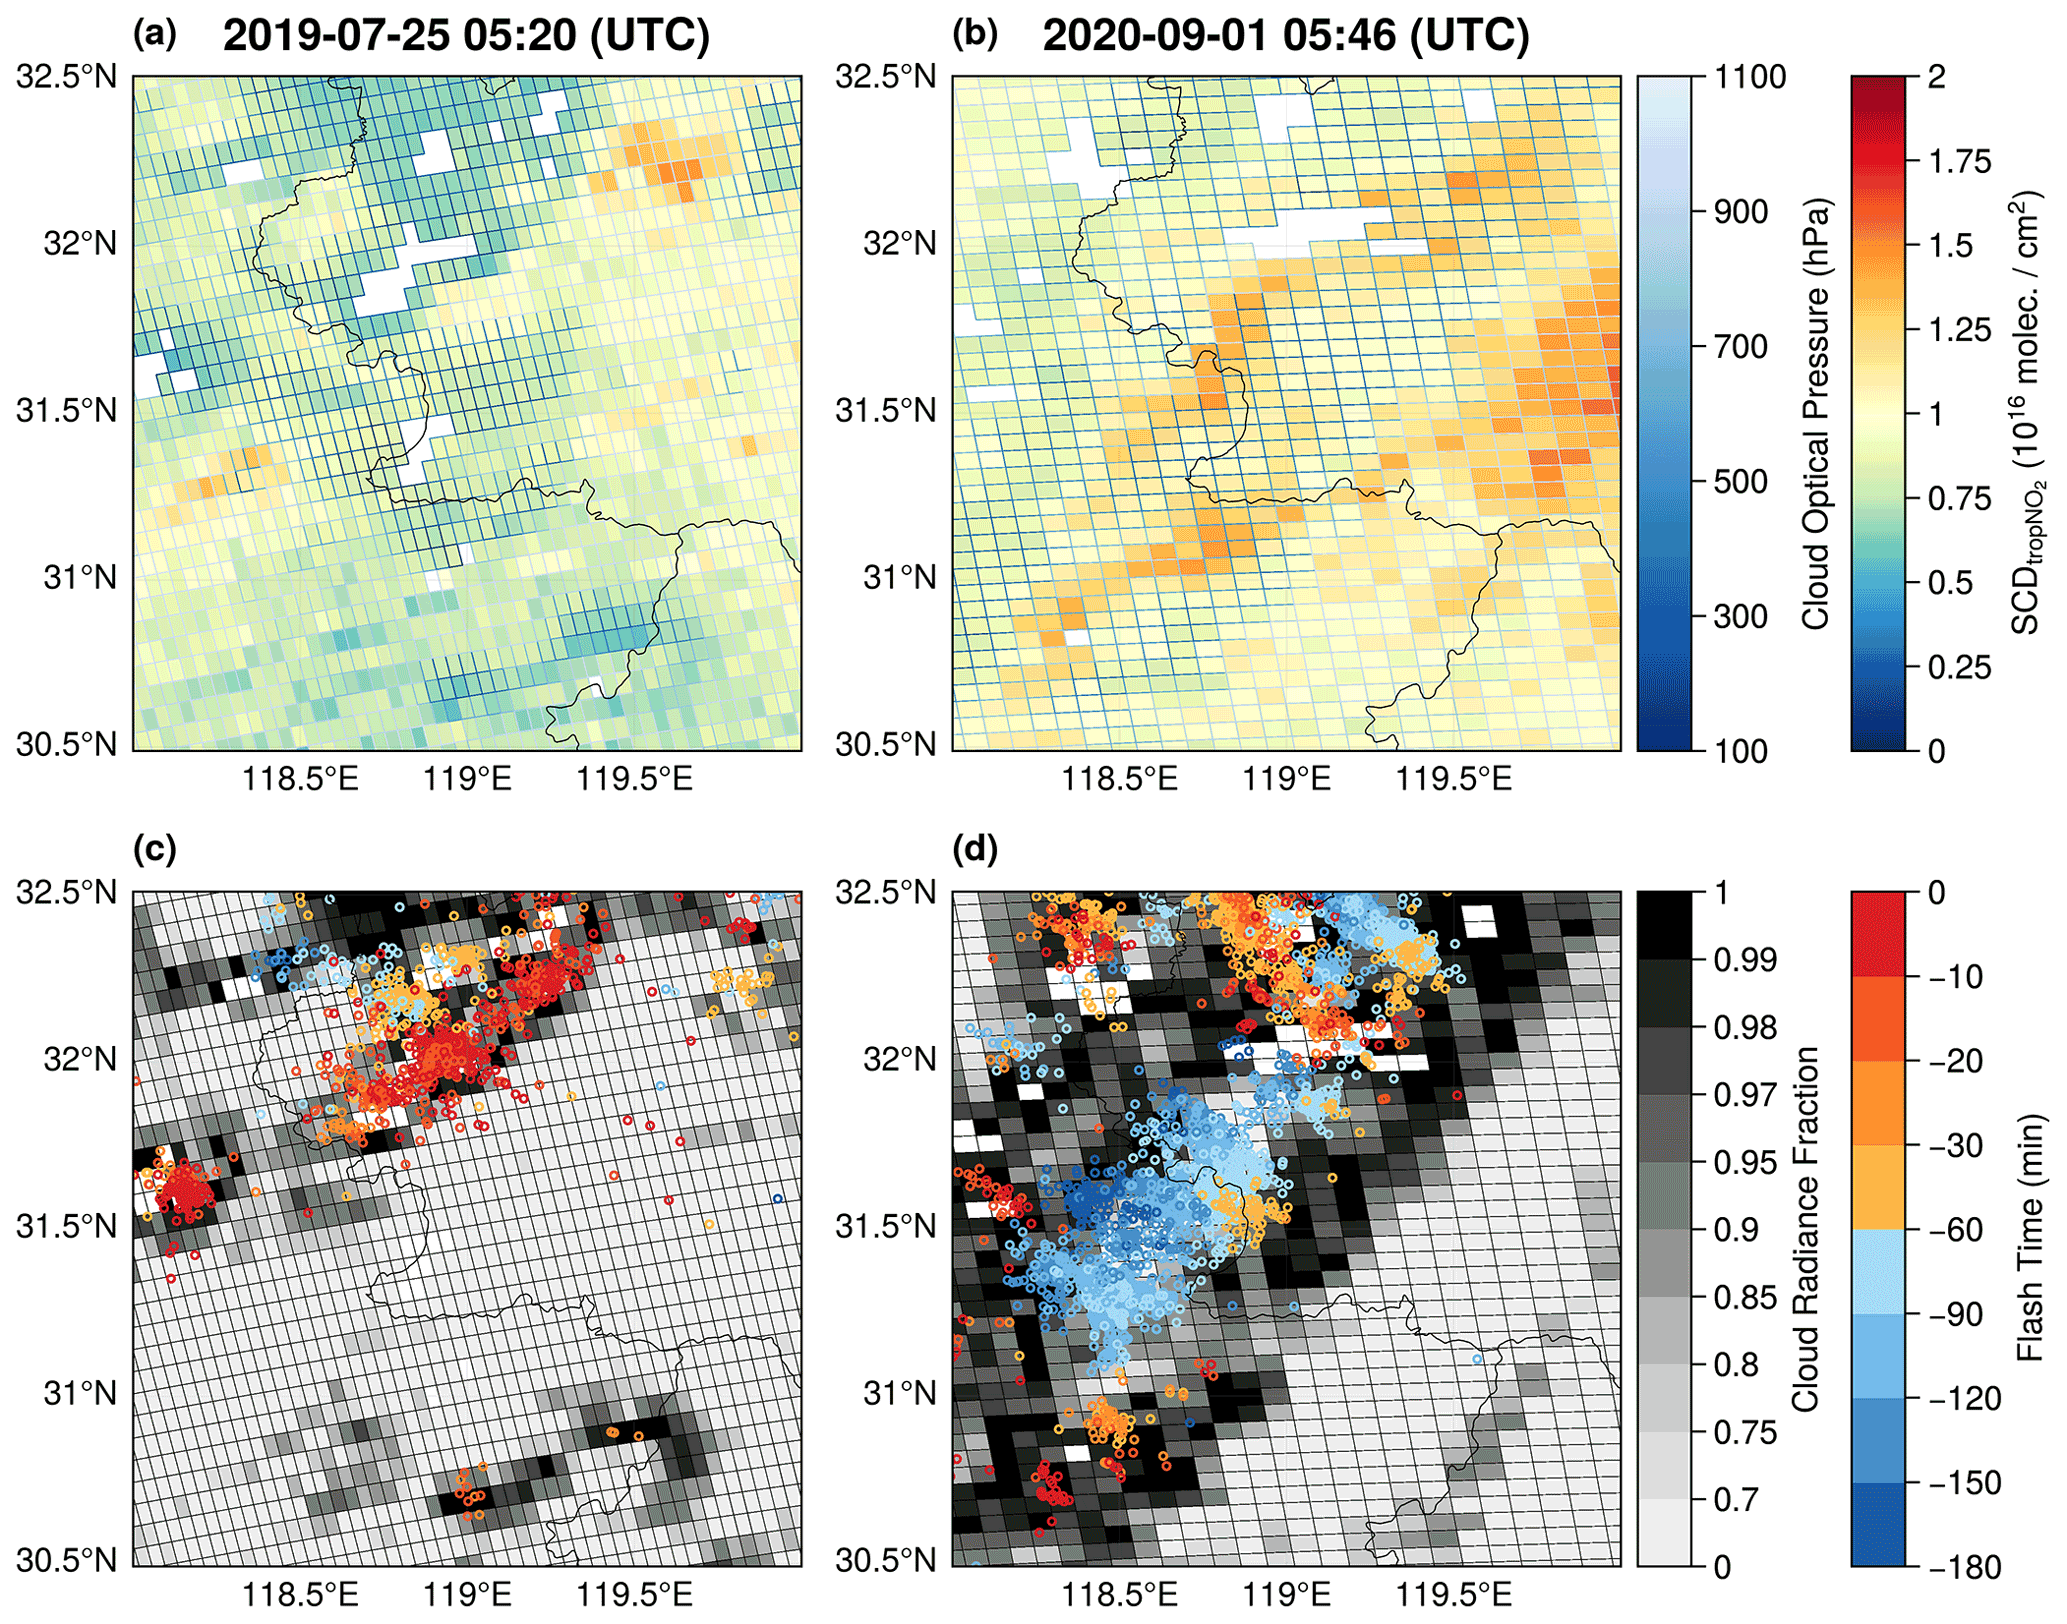
\includegraphics[width=12cm]{./figures/flash_scd.png}
    \caption{
    2019 年 7 月 25 日(左)和 2020 年 9 月 7 日(右)的个例。
    (a, b) 对流层 NO$_2$ 斜柱密度(SCD$_\textrm{tropNO$_2$}$,填充色)和云压(线条颜色)。
    这些白色网格单元代表缺失的 TROPOMI 数据,黑色实线为江苏省。
     (c, d) NO$_2$ 窗区中的云辐射分数和闪电。闪电的颜色取决于相对于TROPOMI过境的发生时间。\\
    Figure \ref{fig:flash_scd}. Events on 25 July 2019 (left) and 07 September 2020 (right).
    (a, b) The tropospheric NO$_2$ slant column density (SCD$_\textrm{tropNO$_2$}$, filled color) and cloud optical pressure (line color).
    These white grid cells stand for missing TROPOMI data.
    The solid black border is Jiangsu province.
    (c, d) The cloud radiance fraction in the NO$_2$ window and flashes whose color depends on the occurring time relative to the TROPOMI overpass time.
    }
    \label{fig:flash_scd}
\end{figure}


\begin{figure}[h]
    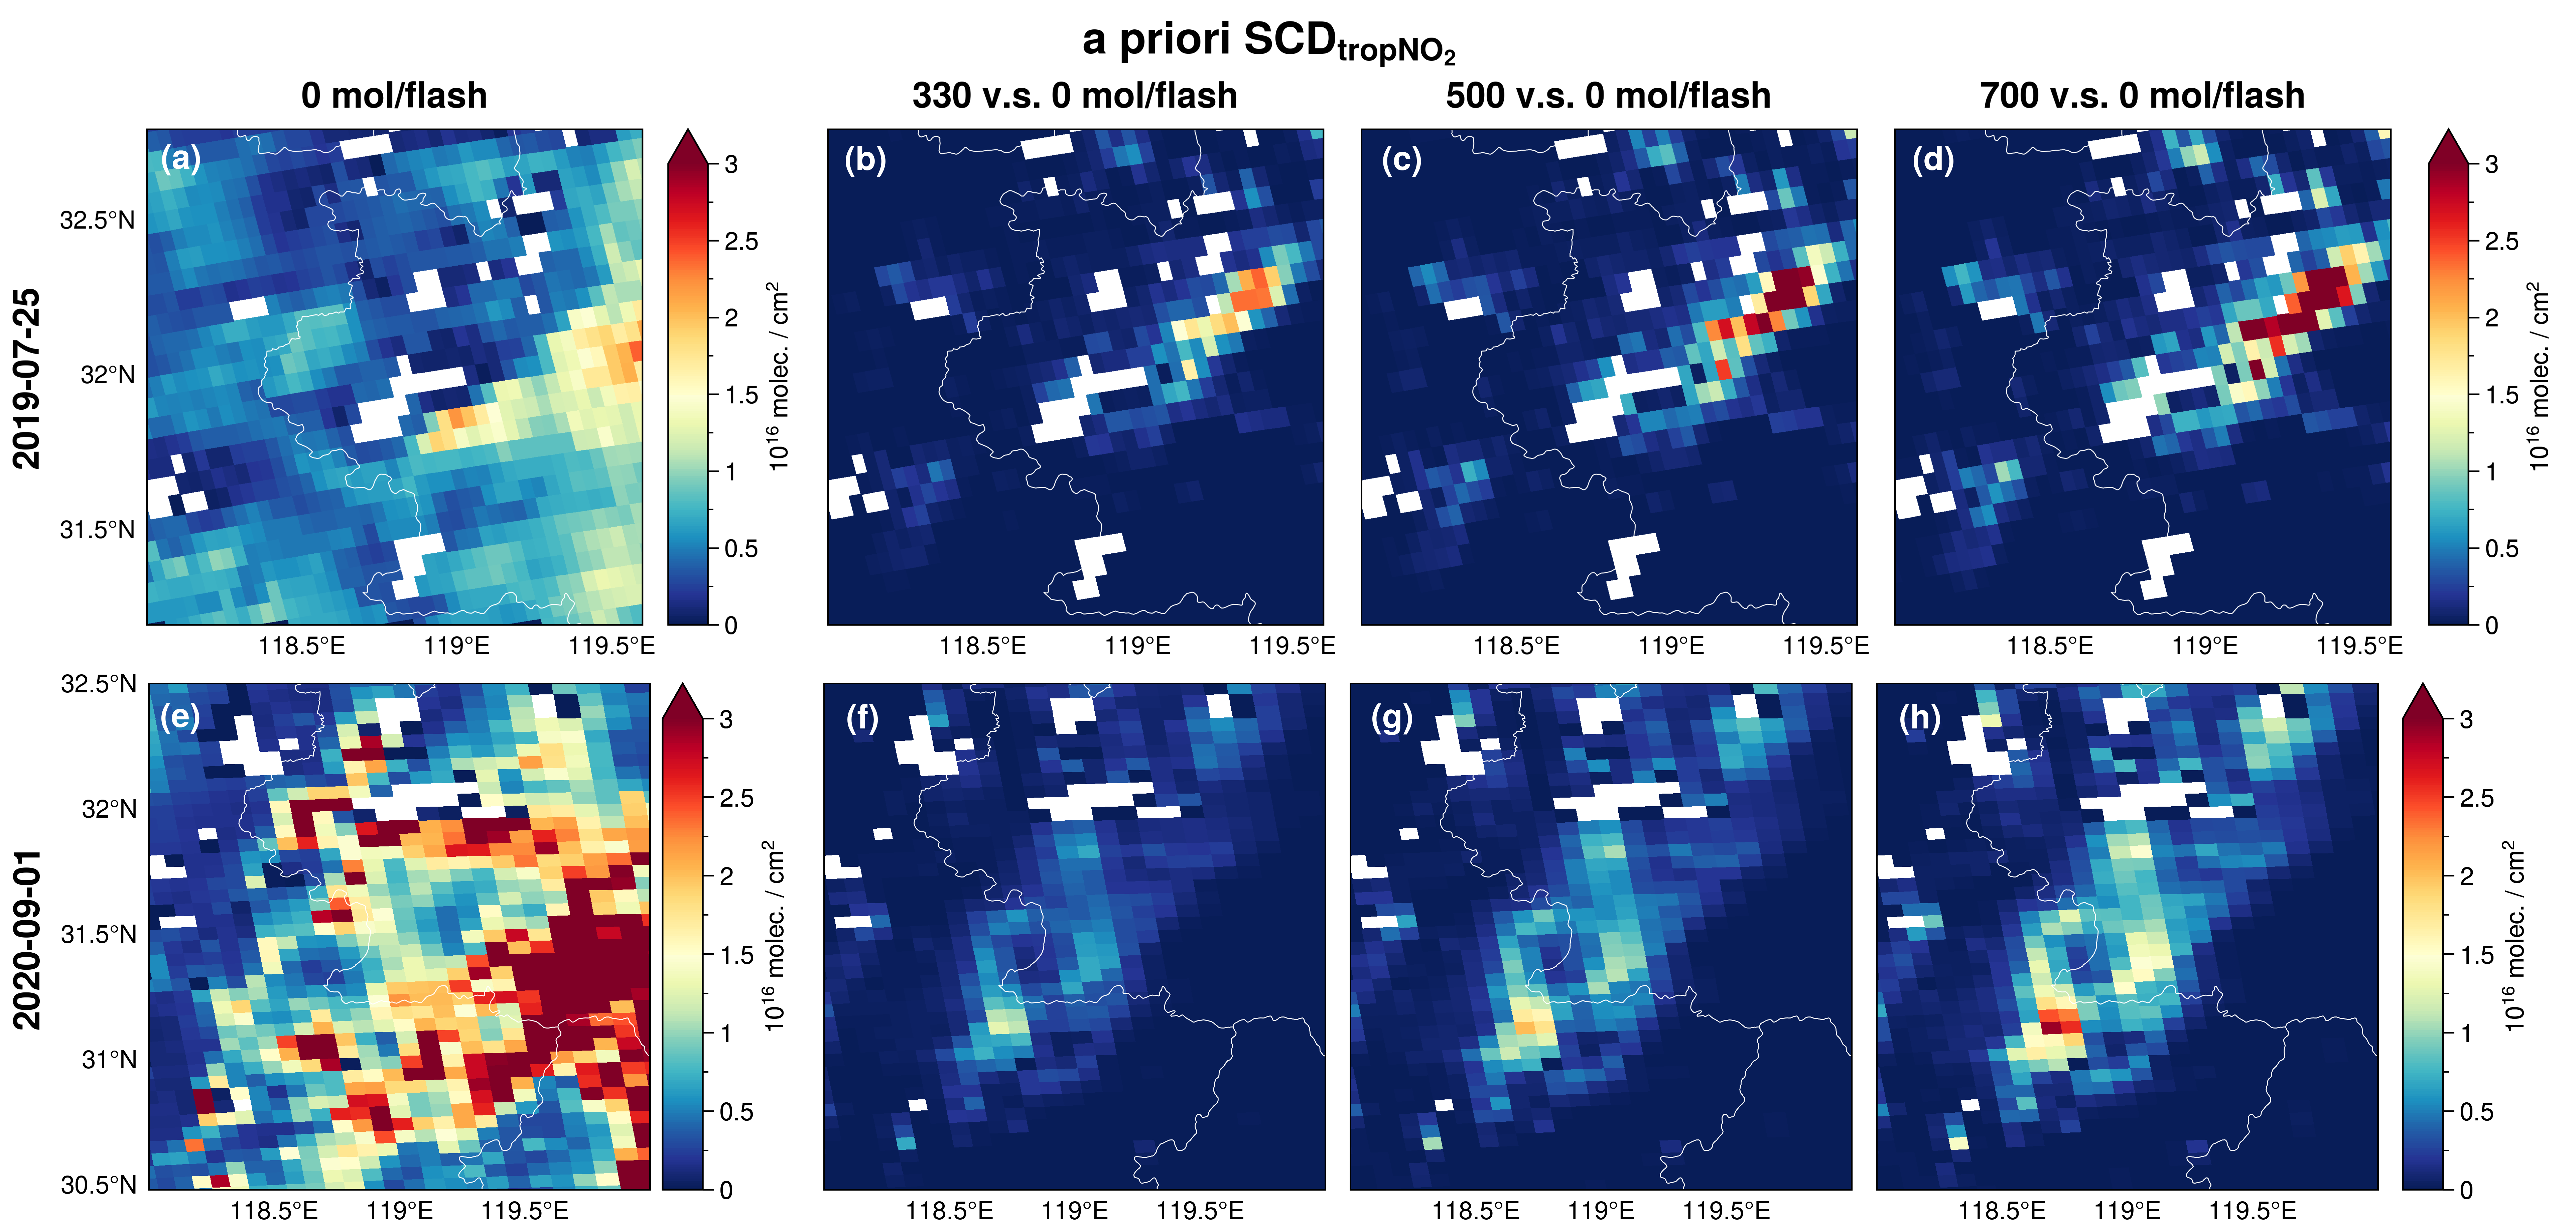
\includegraphics[width=17cm]{./figures/s5p_apriori_scd.png}
    \caption{使用不同闪电NO排放的WRF-Chem结果,重新计算得到的对流层NO$_2$斜柱密度 (SCD$_\textrm{tropNO$_2$}$):
    Figure \ref{fig:s5p_apriori_scd}. (a, e) 0 mol每闪电, (b, f ) 330 mol每闪电, (c, g) 500 mol每闪电 和 (d, h) 700 mol每闪电。\\
    The tropospheric NO$_2$ slant column density (SCD$_\textrm{tropNO$_2$}$) recalculated using the WRF-Chem results with different lightning NO settings: (a, e) 0 mol/flash, (b, f) 330 mol/flash, (c, g) 500 mol/flash and (d, h) 700 mol/flash.
    }
    \label{fig:s5p_apriori_scd}
\end{figure}


\begin{figure}[h]
    \centering
    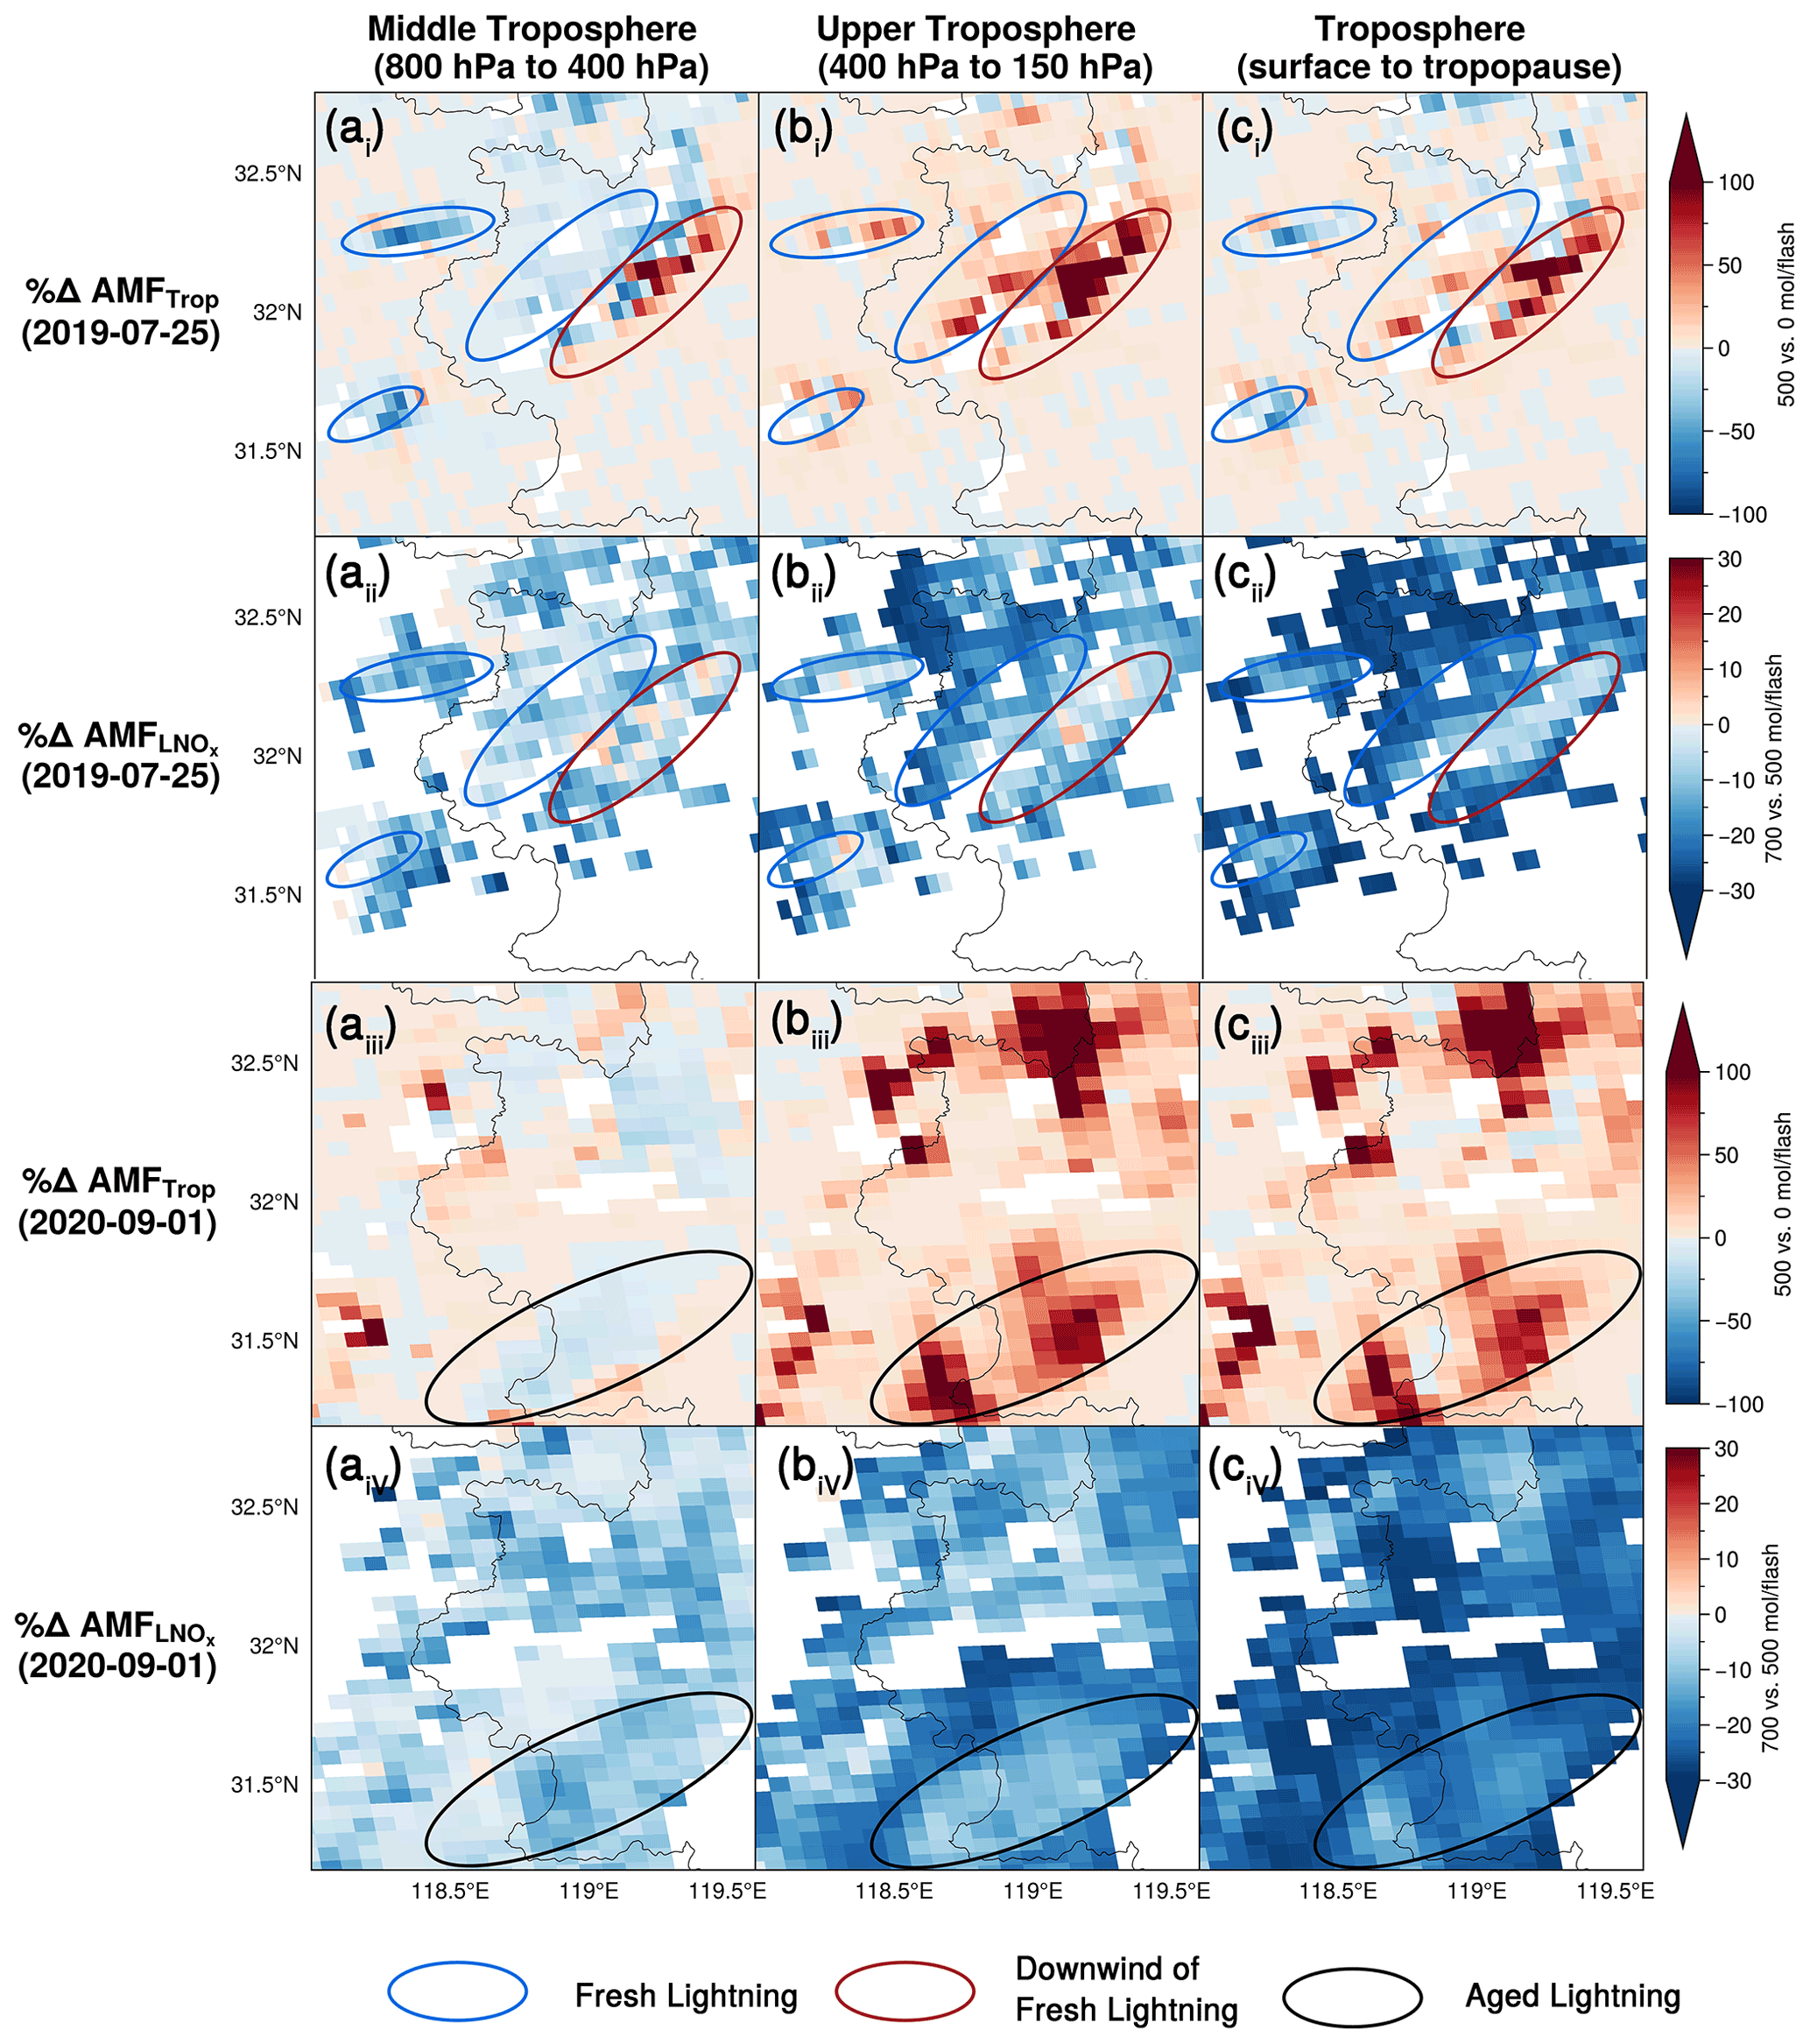
\includegraphics[width=12cm]{./figures/s5p_amf_diff.png}
    \caption{
    通过替换三层的NO$_2$先验廓线,得到的空气质量因子(AMF)百分比差异:三层具体为:对流层中层(左)、对流层上层(中)和整个对流层(右)。
     $\Delta$AMF$_\textrm{trop}$ 是 500 mol NO/闪电得到的AMF$_\textrm{trop}$ 与0 mol NO/闪电得到的AMF$_\textrm{trop}$之差。
     $\Delta$AMF$_\textrm{LNO$_x$}$ 是 500 mol NO/闪电得到的AMF$_\textrm{LNO$_x$}$ 与0 mol NO/闪电得到的AMF$_\textrm{LNO$_x$}$之差。
     标注了三个区域:新生闪电区(蓝色),闪电下风向(红色),和闪电老化区(黑色)。\\
    Figure \ref{fig:s5p_amf_diff}. The percent differences of AMFs by replacing the a priori NO$_2$ profiles at three layers:
    middle troposphere (left), upper troposphere (middle), and troposphere (right).
    $\Delta$AMF$_\textrm{trop}$ is the comparison of the AMF$_\textrm{trop}$ with 500 mol NO per flash relative to 0 mol NO per flash.
    $\Delta$AMF$_\textrm{LNO$_x$}$ is the comparison of the AMF$_\textrm{LNO$_x$}$ with 700 mol NO per flash relative to 500 mol NO per flash.
    Three regions are annotated: fresh lightning (blue),
    downwind of fresh lightning (red),
    and aged lightning (black).
    % Because of the quite large AMF$_\textrm{LNO$_x$}$ values in pixels with little lightning,
    % $\Delta$AMF$_\textrm{LNO$_x$}$ is shown over pixels where 0 $<$ AMF$_\textrm{LNO$_x$}$ $<$ 10.
    }
    \label{fig:s5p_amf_diff}
\end{figure}


\begin{figure}[h]
    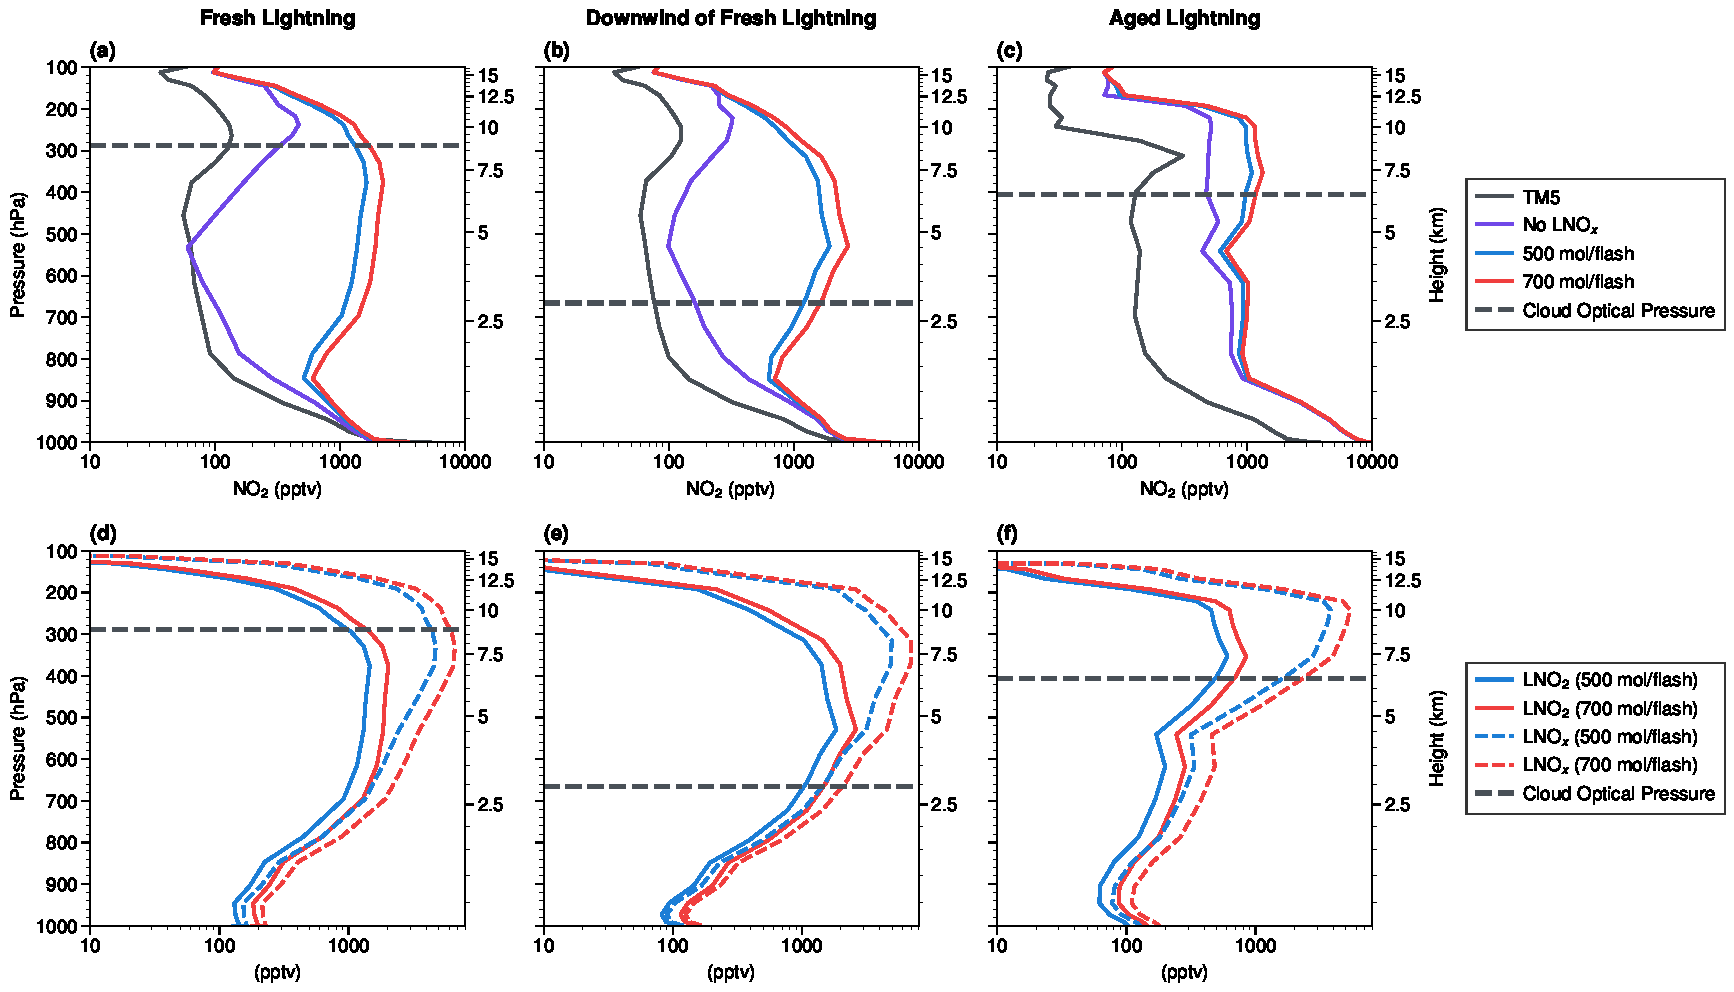
\includegraphics[width=17cm]{./figures/nox_profile.pdf}
    \caption{
    TROPOMI过境时,在不同闪电NO的排放条件下,三个区域(新生闪电区,闪电下风向,和闪电老化区)的各物质垂直廓线。
     (a--c) NO$_2$廓线与官方TM5先验NO$_2$廓线之间的比较。
     (d--f) 闪电 NO$_2$ 和 NO$_x$廓线。灰色虚线是TROPOMI探测到的云压。\\
     Figure \ref{fig:nox_profile}. Profiles with different lightning NO productions at TROPOMI overpass time over three regions (fresh lightning, downwind of fresh lightning, and aged lightning).
    (a--c) The NO$_2$ profiles compared with the official TM5 a priori NO$_2$ profile.
    (d--f) The lightning NO$_2$ and NO$_x$ profiles.
    The gray dashed line is the cloud optical pressure detected by TROPOMI.
    }
    \label{fig:nox_profile}
\end{figure}


\begin{figure}[h]
    \centering
    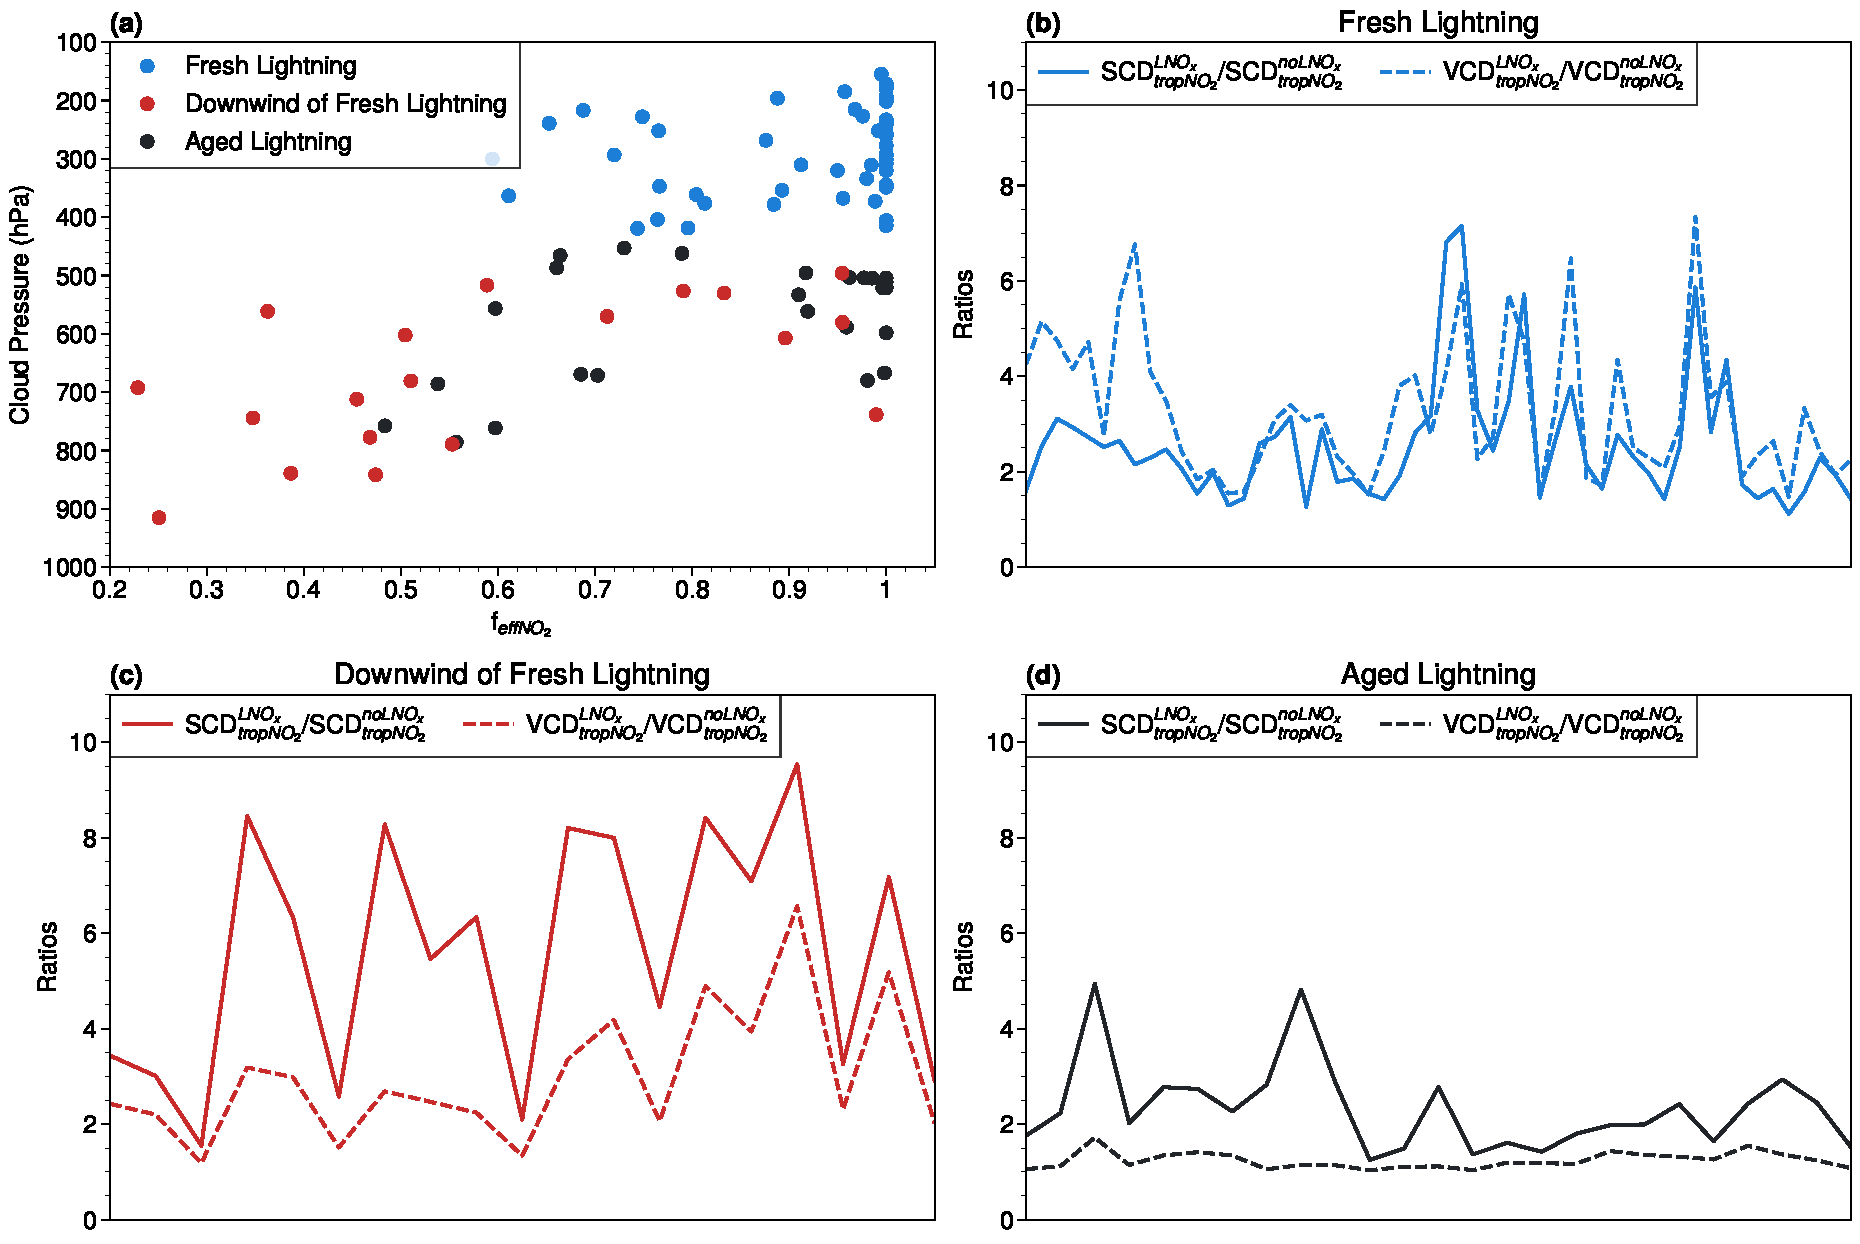
\includegraphics[width=14cm]{./figures/amf_contribution.pdf}
    \caption{
    (a) 图 \ref{fig:s5p_amf_diff} 中定义的三个区域(新生闪电区,闪电下风向,和闪电老化区)的云压和云辐射分数之间的关系。
     (b--d) 这三个区域的先验SCD$^{\textrm{LNO$_x$}}_{\textrm{tropNO$_2$}}$/SCD$^{\textrm{noLNO$_x$}}_{ \textrm{tropNO$_2$}}$和先验VCD$^{\textrm{LNO$_x$}}_{\textrm{tropNO$_2$}}$/VCD$^{\textrm{noLNO$_x$ }}_{\textrm{tropNO$_2$}}$。
     LNO$_x$的上标表示先验变量是通过开启LNO$_x$排放(每次闪光 500 mol NO)计算得到的,而上标为noLNO$_x$则代表未开启LNO$_x$排放。\\
     Figure \ref{fig:amf_contribution}. (a) The relationship between cloud pressure and cloud radiance fraction for three regions defined in Fig. \ref{fig:s5p_amf_diff}: fresh lightning region, downwind of fresh lightning, and aged lightning area.
    (b--d) The a priori SCD$^{\textrm{LNO$_x$}}_{\textrm{tropNO$_2$}}$/SCD$^{\textrm{noLNO$_x$}}_{\textrm{tropNO$_2$}}$ and a priori VCD$^{\textrm{LNO$_x$}}_{\textrm{tropNO$_2$}}$/VCD$^{\textrm{noLNO$_x$}}_{\textrm{tropNO$_2$}}$ of pixels in these three regions. The LNO$_x$ superscript indicates that the a priori variable is calculated with LNO$_x$ (500 mol NO per flash) and the noLNO$_x$ superscript is without LNO$_x$.
    }
    \label{fig:amf_contribution}
\end{figure}


\section{本章小结}
